% Created by tikzDevice version 0.12.3.1 on 2021-02-12 17:49:19
% !TEX encoding = UTF-8 Unicode
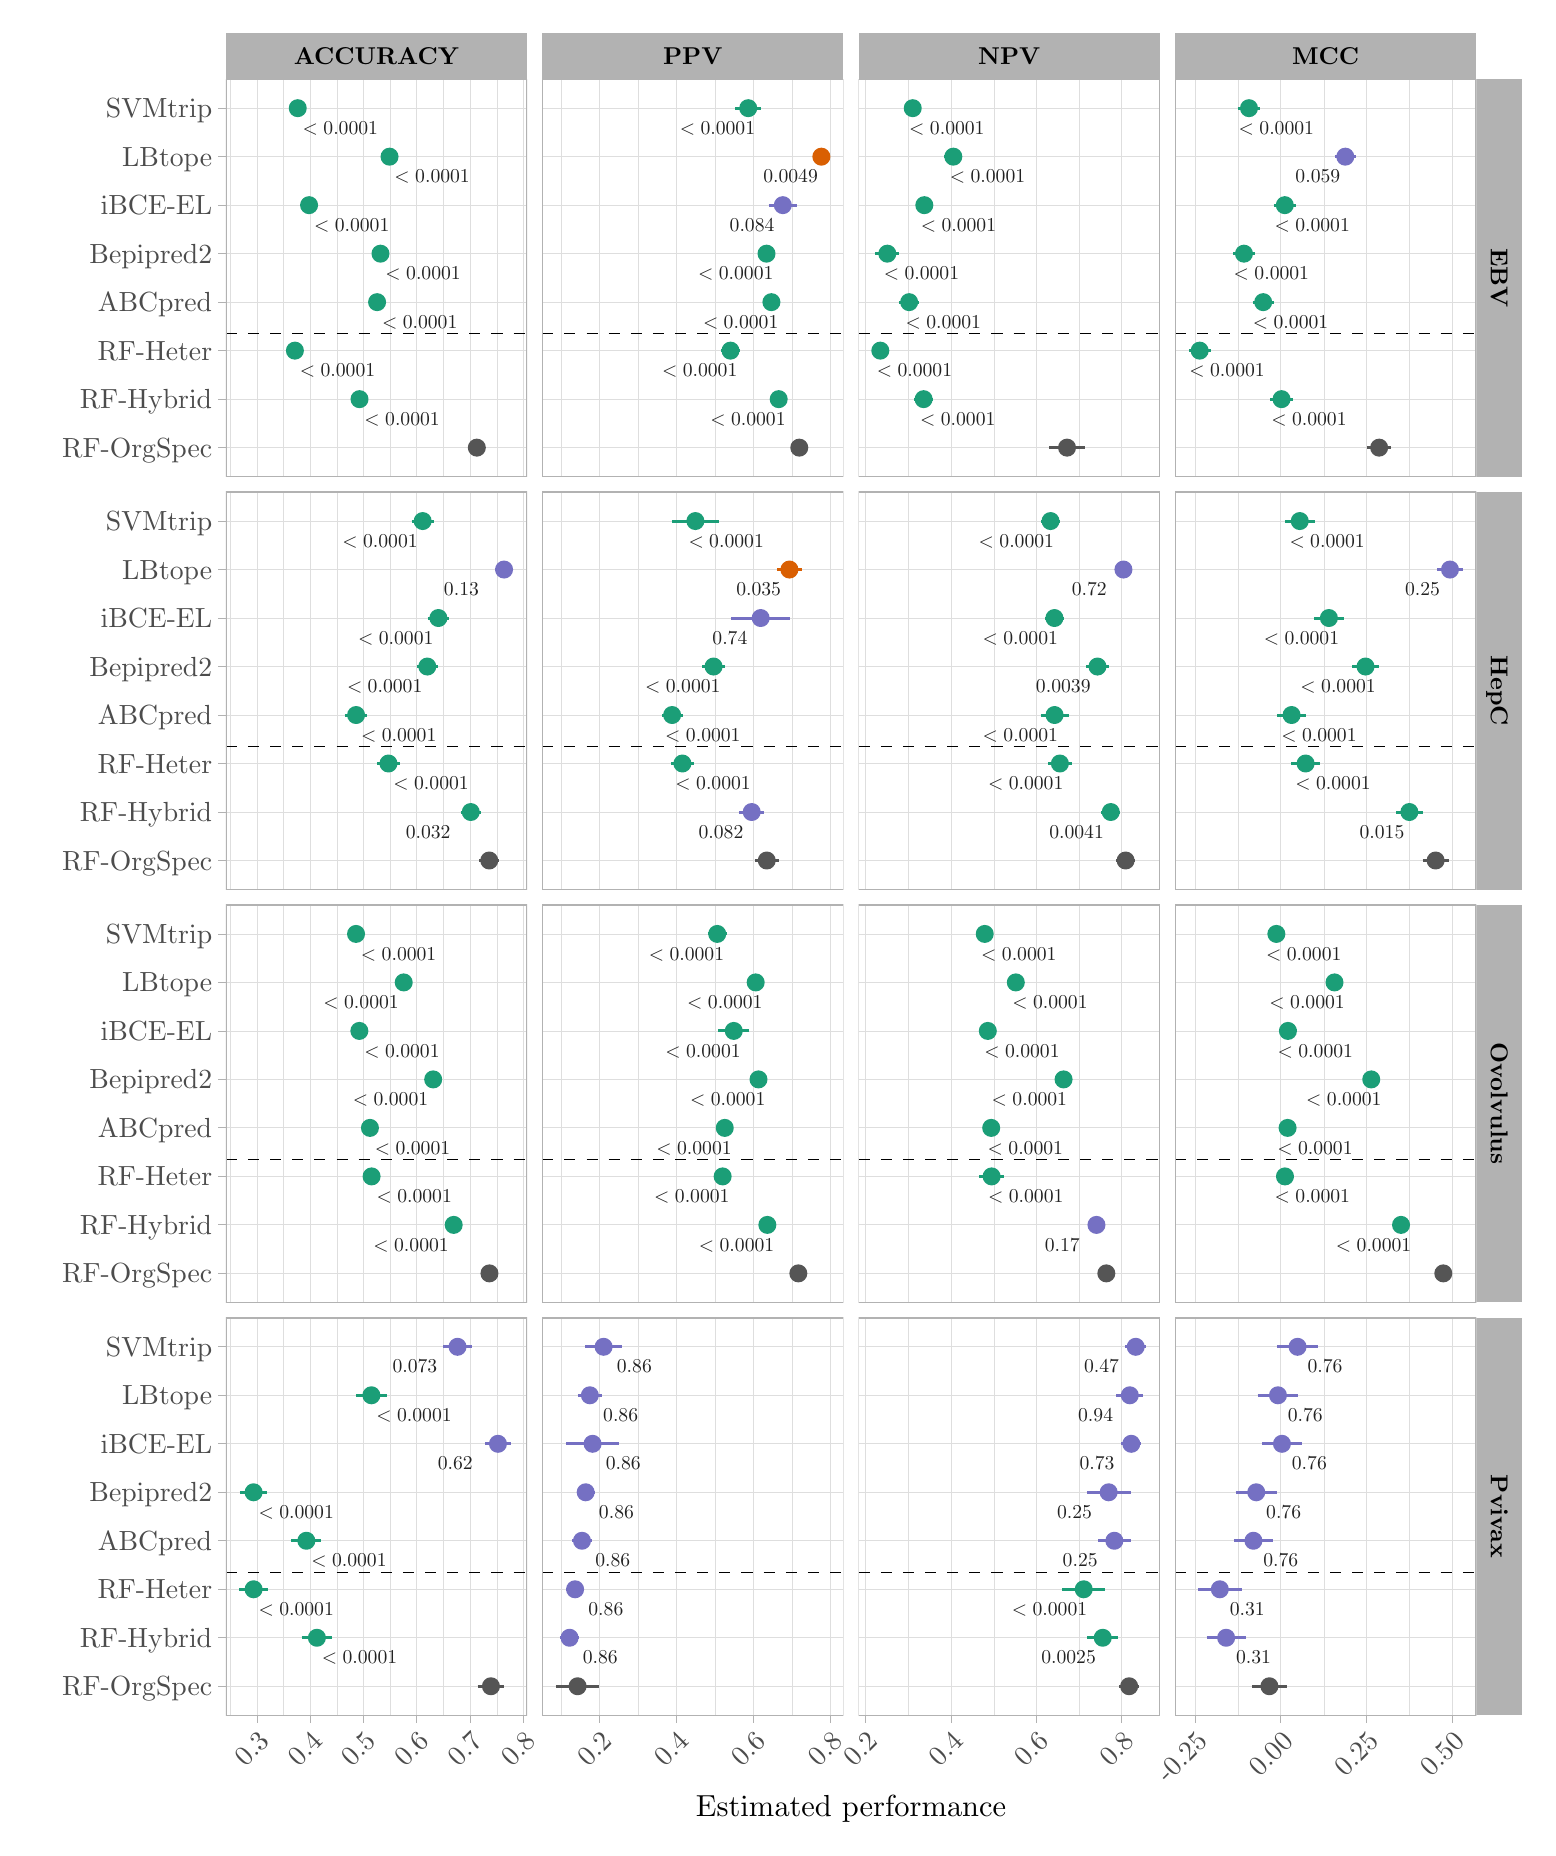
\begin{tikzpicture}[x=1pt,y=1pt]
\definecolor{fillColor}{RGB}{255,255,255}
\path[use as bounding box,fill=fillColor,fill opacity=0.00] (0,0) rectangle (542.02,650.43);
\begin{scope}
\path[clip] (  0.00,  0.00) rectangle (542.02,650.43);
\definecolor{drawColor}{RGB}{255,255,255}
\definecolor{fillColor}{RGB}{255,255,255}

\path[draw=drawColor,line width= 0.6pt,line join=round,line cap=round,fill=fillColor] ( -0.00,  0.00) rectangle (542.02,650.43);
\end{scope}
\begin{scope}
\path[clip] ( 71.60,488.16) rectangle (180.43,631.85);
\definecolor{fillColor}{RGB}{255,255,255}

\path[fill=fillColor] ( 71.60,488.16) rectangle (180.43,631.85);
\definecolor{drawColor}{gray}{0.87}

\path[draw=drawColor,line width= 0.1pt,line join=round] ( 73.22,488.16) --
	( 73.22,631.85);

\path[draw=drawColor,line width= 0.1pt,line join=round] ( 92.47,488.16) --
	( 92.47,631.85);

\path[draw=drawColor,line width= 0.1pt,line join=round] (111.72,488.16) --
	(111.72,631.85);

\path[draw=drawColor,line width= 0.1pt,line join=round] (130.97,488.16) --
	(130.97,631.85);

\path[draw=drawColor,line width= 0.1pt,line join=round] (150.22,488.16) --
	(150.22,631.85);

\path[draw=drawColor,line width= 0.1pt,line join=round] (169.47,488.16) --
	(169.47,631.85);

\path[draw=drawColor,line width= 0.3pt,line join=round] ( 71.60,498.67) --
	(180.43,498.67);

\path[draw=drawColor,line width= 0.3pt,line join=round] ( 71.60,516.19) --
	(180.43,516.19);

\path[draw=drawColor,line width= 0.3pt,line join=round] ( 71.60,533.72) --
	(180.43,533.72);

\path[draw=drawColor,line width= 0.3pt,line join=round] ( 71.60,551.24) --
	(180.43,551.24);

\path[draw=drawColor,line width= 0.3pt,line join=round] ( 71.60,568.76) --
	(180.43,568.76);

\path[draw=drawColor,line width= 0.3pt,line join=round] ( 71.60,586.29) --
	(180.43,586.29);

\path[draw=drawColor,line width= 0.3pt,line join=round] ( 71.60,603.81) --
	(180.43,603.81);

\path[draw=drawColor,line width= 0.3pt,line join=round] ( 71.60,621.33) --
	(180.43,621.33);

\path[draw=drawColor,line width= 0.3pt,line join=round] ( 82.84,488.16) --
	( 82.84,631.85);

\path[draw=drawColor,line width= 0.3pt,line join=round] (102.09,488.16) --
	(102.09,631.85);

\path[draw=drawColor,line width= 0.3pt,line join=round] (121.34,488.16) --
	(121.34,631.85);

\path[draw=drawColor,line width= 0.3pt,line join=round] (140.59,488.16) --
	(140.59,631.85);

\path[draw=drawColor,line width= 0.3pt,line join=round] (159.84,488.16) --
	(159.84,631.85);

\path[draw=drawColor,line width= 0.3pt,line join=round] (179.09,488.16) --
	(179.09,631.85);
\definecolor{drawColor}{RGB}{85,85,85}

\path[draw=drawColor,line width= 1.1pt,line join=round] (159.41,498.67) -- (165.19,498.67);
\definecolor{drawColor}{RGB}{27,158,119}

\path[draw=drawColor,line width= 1.1pt,line join=round] (116.71,516.19) -- (123.11,516.19);

\path[draw=drawColor,line width= 1.1pt,line join=round] ( 93.53,533.72) -- ( 99.60,533.72);

\path[draw=drawColor,line width= 1.1pt,line join=round] (123.25,551.24) -- (129.27,551.24);

\path[draw=drawColor,line width= 1.1pt,line join=round] (124.27,568.76) -- (130.70,568.76);

\path[draw=drawColor,line width= 1.1pt,line join=round] ( 98.63,586.29) -- (104.73,586.29);

\path[draw=drawColor,line width= 1.1pt,line join=round] (127.58,603.81) -- (133.95,603.81);

\path[draw=drawColor,line width= 1.1pt,line join=round] ( 94.59,621.33) -- (100.58,621.33);
\definecolor{drawColor}{RGB}{85,85,85}
\definecolor{fillColor}{RGB}{85,85,85}

\path[draw=drawColor,line width= 0.8pt,line join=round,line cap=round,fill=fillColor] (162.30,498.67) circle (  2.85);
\definecolor{drawColor}{RGB}{27,158,119}
\definecolor{fillColor}{RGB}{27,158,119}

\path[draw=drawColor,line width= 0.8pt,line join=round,line cap=round,fill=fillColor] (119.91,516.19) circle (  2.85);

\path[draw=drawColor,line width= 0.8pt,line join=round,line cap=round,fill=fillColor] ( 96.56,533.72) circle (  2.85);

\path[draw=drawColor,line width= 0.8pt,line join=round,line cap=round,fill=fillColor] (126.26,551.24) circle (  2.85);

\path[draw=drawColor,line width= 0.8pt,line join=round,line cap=round,fill=fillColor] (127.49,568.76) circle (  2.85);

\path[draw=drawColor,line width= 0.8pt,line join=round,line cap=round,fill=fillColor] (101.68,586.29) circle (  2.85);

\path[draw=drawColor,line width= 0.8pt,line join=round,line cap=round,fill=fillColor] (130.76,603.81) circle (  2.85);

\path[draw=drawColor,line width= 0.8pt,line join=round,line cap=round,fill=fillColor] ( 97.59,621.33) circle (  2.85);
\definecolor{drawColor}{RGB}{34,34,34}

\node[text=drawColor,anchor=base,inner sep=0pt, outer sep=0pt, scale=  0.71] at (135.31,506.73) {$<0.0001$};

\node[text=drawColor,anchor=base,inner sep=0pt, outer sep=0pt, scale=  0.71] at (111.96,524.26) {$<0.0001$};

\node[text=drawColor,anchor=base,inner sep=0pt, outer sep=0pt, scale=  0.71] at (141.66,541.78) {$<0.0001$};

\node[text=drawColor,anchor=base,inner sep=0pt, outer sep=0pt, scale=  0.71] at (142.89,559.30) {$<0.0001$};

\node[text=drawColor,anchor=base,inner sep=0pt, outer sep=0pt, scale=  0.71] at (117.08,576.83) {$<0.0001$};

\node[text=drawColor,anchor=base,inner sep=0pt, outer sep=0pt, scale=  0.71] at (146.16,594.35) {$<0.0001$};

\node[text=drawColor,anchor=base,inner sep=0pt, outer sep=0pt, scale=  0.71] at (112.99,611.87) {$<0.0001$};
\definecolor{drawColor}{RGB}{0,0,0}

\path[draw=drawColor,line width= 0.2pt,dash pattern=on 4pt off 4pt ,line join=round] ( 71.60,539.85) -- (180.43,539.85);
\definecolor{drawColor}{gray}{0.70}

\path[draw=drawColor,line width= 0.6pt,line join=round,line cap=round] ( 71.60,488.16) rectangle (180.43,631.85);
\end{scope}
\begin{scope}
\path[clip] ( 71.60,338.96) rectangle (180.43,482.66);
\definecolor{fillColor}{RGB}{255,255,255}

\path[fill=fillColor] ( 71.60,338.96) rectangle (180.43,482.66);
\definecolor{drawColor}{gray}{0.87}

\path[draw=drawColor,line width= 0.1pt,line join=round] ( 73.22,338.96) --
	( 73.22,482.66);

\path[draw=drawColor,line width= 0.1pt,line join=round] ( 92.47,338.96) --
	( 92.47,482.66);

\path[draw=drawColor,line width= 0.1pt,line join=round] (111.72,338.96) --
	(111.72,482.66);

\path[draw=drawColor,line width= 0.1pt,line join=round] (130.97,338.96) --
	(130.97,482.66);

\path[draw=drawColor,line width= 0.1pt,line join=round] (150.22,338.96) --
	(150.22,482.66);

\path[draw=drawColor,line width= 0.1pt,line join=round] (169.47,338.96) --
	(169.47,482.66);

\path[draw=drawColor,line width= 0.3pt,line join=round] ( 71.60,349.48) --
	(180.43,349.48);

\path[draw=drawColor,line width= 0.3pt,line join=round] ( 71.60,367.00) --
	(180.43,367.00);

\path[draw=drawColor,line width= 0.3pt,line join=round] ( 71.60,384.53) --
	(180.43,384.53);

\path[draw=drawColor,line width= 0.3pt,line join=round] ( 71.60,402.05) --
	(180.43,402.05);

\path[draw=drawColor,line width= 0.3pt,line join=round] ( 71.60,419.57) --
	(180.43,419.57);

\path[draw=drawColor,line width= 0.3pt,line join=round] ( 71.60,437.10) --
	(180.43,437.10);

\path[draw=drawColor,line width= 0.3pt,line join=round] ( 71.60,454.62) --
	(180.43,454.62);

\path[draw=drawColor,line width= 0.3pt,line join=round] ( 71.60,472.14) --
	(180.43,472.14);

\path[draw=drawColor,line width= 0.3pt,line join=round] ( 82.84,338.96) --
	( 82.84,482.66);

\path[draw=drawColor,line width= 0.3pt,line join=round] (102.09,338.96) --
	(102.09,482.66);

\path[draw=drawColor,line width= 0.3pt,line join=round] (121.34,338.96) --
	(121.34,482.66);

\path[draw=drawColor,line width= 0.3pt,line join=round] (140.59,338.96) --
	(140.59,482.66);

\path[draw=drawColor,line width= 0.3pt,line join=round] (159.84,338.96) --
	(159.84,482.66);

\path[draw=drawColor,line width= 0.3pt,line join=round] (179.09,338.96) --
	(179.09,482.66);
\definecolor{drawColor}{RGB}{85,85,85}

\path[draw=drawColor,line width= 1.1pt,line join=round] (163.25,349.48) -- (170.33,349.48);
\definecolor{drawColor}{RGB}{27,158,119}

\path[draw=drawColor,line width= 1.1pt,line join=round] (156.47,367.00) -- (163.75,367.00);

\path[draw=drawColor,line width= 1.1pt,line join=round] (126.33,384.53) -- (134.40,384.53);

\path[draw=drawColor,line width= 1.1pt,line join=round] (114.57,402.05) -- (122.76,402.05);

\path[draw=drawColor,line width= 1.1pt,line join=round] (140.60,419.57) -- (148.20,419.57);

\path[draw=drawColor,line width= 1.1pt,line join=round] (144.49,437.10) -- (152.34,437.10);
\definecolor{drawColor}{RGB}{117,112,195}

\path[draw=drawColor,line width= 1.1pt,line join=round] (168.80,454.62) -- (175.48,454.62);
\definecolor{drawColor}{RGB}{27,158,119}

\path[draw=drawColor,line width= 1.1pt,line join=round] (138.73,472.14) -- (146.74,472.14);
\definecolor{drawColor}{RGB}{85,85,85}
\definecolor{fillColor}{RGB}{85,85,85}

\path[draw=drawColor,line width= 0.8pt,line join=round,line cap=round,fill=fillColor] (166.79,349.48) circle (  2.85);
\definecolor{drawColor}{RGB}{27,158,119}
\definecolor{fillColor}{RGB}{27,158,119}

\path[draw=drawColor,line width= 0.8pt,line join=round,line cap=round,fill=fillColor] (160.11,367.00) circle (  2.85);

\path[draw=drawColor,line width= 0.8pt,line join=round,line cap=round,fill=fillColor] (130.37,384.53) circle (  2.85);

\path[draw=drawColor,line width= 0.8pt,line join=round,line cap=round,fill=fillColor] (118.67,402.05) circle (  2.85);

\path[draw=drawColor,line width= 0.8pt,line join=round,line cap=round,fill=fillColor] (144.40,419.57) circle (  2.85);

\path[draw=drawColor,line width= 0.8pt,line join=round,line cap=round,fill=fillColor] (148.41,437.10) circle (  2.85);
\definecolor{drawColor}{RGB}{117,112,195}
\definecolor{fillColor}{RGB}{117,112,195}

\path[draw=drawColor,line width= 0.8pt,line join=round,line cap=round,fill=fillColor] (172.14,454.62) circle (  2.85);
\definecolor{drawColor}{RGB}{27,158,119}
\definecolor{fillColor}{RGB}{27,158,119}

\path[draw=drawColor,line width= 0.8pt,line join=round,line cap=round,fill=fillColor] (142.73,472.14) circle (  2.85);
\definecolor{drawColor}{RGB}{34,34,34}

\node[text=drawColor,anchor=base,inner sep=0pt, outer sep=0pt, scale=  0.71] at (144.71,357.54) {0.032};

\node[text=drawColor,anchor=base,inner sep=0pt, outer sep=0pt, scale=  0.71] at (145.77,375.07) {$<0.0001$};

\node[text=drawColor,anchor=base,inner sep=0pt, outer sep=0pt, scale=  0.71] at (134.07,392.59) {$<0.0001$};

\node[text=drawColor,anchor=base,inner sep=0pt, outer sep=0pt, scale=  0.71] at (129.00,410.11) {$<0.0001$};

\node[text=drawColor,anchor=base,inner sep=0pt, outer sep=0pt, scale=  0.71] at (133.01,427.64) {$<0.0001$};

\node[text=drawColor,anchor=base,inner sep=0pt, outer sep=0pt, scale=  0.71] at (156.74,445.16) {0.13};

\node[text=drawColor,anchor=base,inner sep=0pt, outer sep=0pt, scale=  0.71] at (127.33,462.68) {$<0.0001$};
\definecolor{drawColor}{RGB}{0,0,0}

\path[draw=drawColor,line width= 0.2pt,dash pattern=on 4pt off 4pt ,line join=round] ( 71.60,390.66) -- (180.43,390.66);
\definecolor{drawColor}{gray}{0.70}

\path[draw=drawColor,line width= 0.6pt,line join=round,line cap=round] ( 71.60,338.96) rectangle (180.43,482.66);
\end{scope}
\begin{scope}
\path[clip] ( 71.60,189.77) rectangle (180.43,333.46);
\definecolor{fillColor}{RGB}{255,255,255}

\path[fill=fillColor] ( 71.60,189.77) rectangle (180.43,333.46);
\definecolor{drawColor}{gray}{0.87}

\path[draw=drawColor,line width= 0.1pt,line join=round] ( 73.22,189.77) --
	( 73.22,333.46);

\path[draw=drawColor,line width= 0.1pt,line join=round] ( 92.47,189.77) --
	( 92.47,333.46);

\path[draw=drawColor,line width= 0.1pt,line join=round] (111.72,189.77) --
	(111.72,333.46);

\path[draw=drawColor,line width= 0.1pt,line join=round] (130.97,189.77) --
	(130.97,333.46);

\path[draw=drawColor,line width= 0.1pt,line join=round] (150.22,189.77) --
	(150.22,333.46);

\path[draw=drawColor,line width= 0.1pt,line join=round] (169.47,189.77) --
	(169.47,333.46);

\path[draw=drawColor,line width= 0.3pt,line join=round] ( 71.60,200.29) --
	(180.43,200.29);

\path[draw=drawColor,line width= 0.3pt,line join=round] ( 71.60,217.81) --
	(180.43,217.81);

\path[draw=drawColor,line width= 0.3pt,line join=round] ( 71.60,235.33) --
	(180.43,235.33);

\path[draw=drawColor,line width= 0.3pt,line join=round] ( 71.60,252.86) --
	(180.43,252.86);

\path[draw=drawColor,line width= 0.3pt,line join=round] ( 71.60,270.38) --
	(180.43,270.38);

\path[draw=drawColor,line width= 0.3pt,line join=round] ( 71.60,287.90) --
	(180.43,287.90);

\path[draw=drawColor,line width= 0.3pt,line join=round] ( 71.60,305.43) --
	(180.43,305.43);

\path[draw=drawColor,line width= 0.3pt,line join=round] ( 71.60,322.95) --
	(180.43,322.95);

\path[draw=drawColor,line width= 0.3pt,line join=round] ( 82.84,189.77) --
	( 82.84,333.46);

\path[draw=drawColor,line width= 0.3pt,line join=round] (102.09,189.77) --
	(102.09,333.46);

\path[draw=drawColor,line width= 0.3pt,line join=round] (121.34,189.77) --
	(121.34,333.46);

\path[draw=drawColor,line width= 0.3pt,line join=round] (140.59,189.77) --
	(140.59,333.46);

\path[draw=drawColor,line width= 0.3pt,line join=round] (159.84,189.77) --
	(159.84,333.46);

\path[draw=drawColor,line width= 0.3pt,line join=round] (179.09,189.77) --
	(179.09,333.46);
\definecolor{drawColor}{RGB}{85,85,85}

\path[draw=drawColor,line width= 1.1pt,line join=round] (164.78,200.29) -- (168.95,200.29);
\definecolor{drawColor}{RGB}{27,158,119}

\path[draw=drawColor,line width= 1.1pt,line join=round] (151.65,217.81) -- (156.24,217.81);

\path[draw=drawColor,line width= 1.1pt,line join=round] (121.87,235.33) -- (126.68,235.33);

\path[draw=drawColor,line width= 1.1pt,line join=round] (121.31,252.86) -- (126.04,252.86);

\path[draw=drawColor,line width= 1.1pt,line join=round] (144.10,270.38) -- (148.95,270.38);

\path[draw=drawColor,line width= 1.1pt,line join=round] (117.41,287.90) -- (122.28,287.90);

\path[draw=drawColor,line width= 1.1pt,line join=round] (133.57,305.43) -- (138.18,305.43);

\path[draw=drawColor,line width= 1.1pt,line join=round] (116.13,322.95) -- (121.17,322.95);
\definecolor{drawColor}{RGB}{85,85,85}
\definecolor{fillColor}{RGB}{85,85,85}

\path[draw=drawColor,line width= 0.8pt,line join=round,line cap=round,fill=fillColor] (166.86,200.29) circle (  2.85);
\definecolor{drawColor}{RGB}{27,158,119}
\definecolor{fillColor}{RGB}{27,158,119}

\path[draw=drawColor,line width= 0.8pt,line join=round,line cap=round,fill=fillColor] (153.94,217.81) circle (  2.85);

\path[draw=drawColor,line width= 0.8pt,line join=round,line cap=round,fill=fillColor] (124.27,235.33) circle (  2.85);

\path[draw=drawColor,line width= 0.8pt,line join=round,line cap=round,fill=fillColor] (123.68,252.86) circle (  2.85);

\path[draw=drawColor,line width= 0.8pt,line join=round,line cap=round,fill=fillColor] (146.53,270.38) circle (  2.85);

\path[draw=drawColor,line width= 0.8pt,line join=round,line cap=round,fill=fillColor] (119.85,287.90) circle (  2.85);

\path[draw=drawColor,line width= 0.8pt,line join=round,line cap=round,fill=fillColor] (135.88,305.43) circle (  2.85);

\path[draw=drawColor,line width= 0.8pt,line join=round,line cap=round,fill=fillColor] (118.65,322.95) circle (  2.85);
\definecolor{drawColor}{RGB}{34,34,34}

\node[text=drawColor,anchor=base,inner sep=0pt, outer sep=0pt, scale=  0.71] at (138.54,208.35) {$<0.0001$};

\node[text=drawColor,anchor=base,inner sep=0pt, outer sep=0pt, scale=  0.71] at (139.67,225.88) {$<0.0001$};

\node[text=drawColor,anchor=base,inner sep=0pt, outer sep=0pt, scale=  0.71] at (139.08,243.40) {$<0.0001$};

\node[text=drawColor,anchor=base,inner sep=0pt, outer sep=0pt, scale=  0.71] at (131.13,260.92) {$<0.0001$};

\node[text=drawColor,anchor=base,inner sep=0pt, outer sep=0pt, scale=  0.71] at (135.25,278.45) {$<0.0001$};

\node[text=drawColor,anchor=base,inner sep=0pt, outer sep=0pt, scale=  0.71] at (120.48,295.97) {$<0.0001$};

\node[text=drawColor,anchor=base,inner sep=0pt, outer sep=0pt, scale=  0.71] at (134.05,313.49) {$<0.0001$};
\definecolor{drawColor}{RGB}{0,0,0}

\path[draw=drawColor,line width= 0.2pt,dash pattern=on 4pt off 4pt ,line join=round] ( 71.60,241.47) -- (180.43,241.47);
\definecolor{drawColor}{gray}{0.70}

\path[draw=drawColor,line width= 0.6pt,line join=round,line cap=round] ( 71.60,189.77) rectangle (180.43,333.46);
\end{scope}
\begin{scope}
\path[clip] ( 71.60, 40.58) rectangle (180.43,184.27);
\definecolor{fillColor}{RGB}{255,255,255}

\path[fill=fillColor] ( 71.60, 40.58) rectangle (180.43,184.27);
\definecolor{drawColor}{gray}{0.87}

\path[draw=drawColor,line width= 0.1pt,line join=round] ( 73.22, 40.58) --
	( 73.22,184.27);

\path[draw=drawColor,line width= 0.1pt,line join=round] ( 92.47, 40.58) --
	( 92.47,184.27);

\path[draw=drawColor,line width= 0.1pt,line join=round] (111.72, 40.58) --
	(111.72,184.27);

\path[draw=drawColor,line width= 0.1pt,line join=round] (130.97, 40.58) --
	(130.97,184.27);

\path[draw=drawColor,line width= 0.1pt,line join=round] (150.22, 40.58) --
	(150.22,184.27);

\path[draw=drawColor,line width= 0.1pt,line join=round] (169.47, 40.58) --
	(169.47,184.27);

\path[draw=drawColor,line width= 0.3pt,line join=round] ( 71.60, 51.10) --
	(180.43, 51.10);

\path[draw=drawColor,line width= 0.3pt,line join=round] ( 71.60, 68.62) --
	(180.43, 68.62);

\path[draw=drawColor,line width= 0.3pt,line join=round] ( 71.60, 86.14) --
	(180.43, 86.14);

\path[draw=drawColor,line width= 0.3pt,line join=round] ( 71.60,103.67) --
	(180.43,103.67);

\path[draw=drawColor,line width= 0.3pt,line join=round] ( 71.60,121.19) --
	(180.43,121.19);

\path[draw=drawColor,line width= 0.3pt,line join=round] ( 71.60,138.71) --
	(180.43,138.71);

\path[draw=drawColor,line width= 0.3pt,line join=round] ( 71.60,156.24) --
	(180.43,156.24);

\path[draw=drawColor,line width= 0.3pt,line join=round] ( 71.60,173.76) --
	(180.43,173.76);

\path[draw=drawColor,line width= 0.3pt,line join=round] ( 82.84, 40.58) --
	( 82.84,184.27);

\path[draw=drawColor,line width= 0.3pt,line join=round] (102.09, 40.58) --
	(102.09,184.27);

\path[draw=drawColor,line width= 0.3pt,line join=round] (121.34, 40.58) --
	(121.34,184.27);

\path[draw=drawColor,line width= 0.3pt,line join=round] (140.59, 40.58) --
	(140.59,184.27);

\path[draw=drawColor,line width= 0.3pt,line join=round] (159.84, 40.58) --
	(159.84,184.27);

\path[draw=drawColor,line width= 0.3pt,line join=round] (179.09, 40.58) --
	(179.09,184.27);
\definecolor{drawColor}{RGB}{85,85,85}

\path[draw=drawColor,line width= 1.1pt,line join=round] (162.59, 51.10) -- (172.21, 51.10);
\definecolor{drawColor}{RGB}{27,158,119}

\path[draw=drawColor,line width= 1.1pt,line join=round] ( 98.96, 68.62) -- (110.06, 68.62);

\path[draw=drawColor,line width= 1.1pt,line join=round] ( 76.54, 86.14) -- ( 86.73, 86.14);

\path[draw=drawColor,line width= 1.1pt,line join=round] ( 95.29,103.67) -- (106.10,103.67);

\path[draw=drawColor,line width= 1.1pt,line join=round] ( 76.67,121.19) -- ( 86.60,121.19);
\definecolor{drawColor}{RGB}{117,112,195}

\path[draw=drawColor,line width= 1.1pt,line join=round] (165.31,138.71) -- (174.58,138.71);
\definecolor{drawColor}{RGB}{27,158,119}

\path[draw=drawColor,line width= 1.1pt,line join=round] (118.56,156.24) -- (129.85,156.24);
\definecolor{drawColor}{RGB}{117,112,195}

\path[draw=drawColor,line width= 1.1pt,line join=round] (150.13,173.76) -- (160.53,173.76);
\definecolor{drawColor}{RGB}{85,85,85}
\definecolor{fillColor}{RGB}{85,85,85}

\path[draw=drawColor,line width= 0.8pt,line join=round,line cap=round,fill=fillColor] (167.40, 51.10) circle (  2.85);
\definecolor{drawColor}{RGB}{27,158,119}
\definecolor{fillColor}{RGB}{27,158,119}

\path[draw=drawColor,line width= 0.8pt,line join=round,line cap=round,fill=fillColor] (104.51, 68.62) circle (  2.85);

\path[draw=drawColor,line width= 0.8pt,line join=round,line cap=round,fill=fillColor] ( 81.64, 86.14) circle (  2.85);

\path[draw=drawColor,line width= 0.8pt,line join=round,line cap=round,fill=fillColor] (100.70,103.67) circle (  2.85);

\path[draw=drawColor,line width= 0.8pt,line join=round,line cap=round,fill=fillColor] ( 81.64,121.19) circle (  2.85);
\definecolor{drawColor}{RGB}{117,112,195}
\definecolor{fillColor}{RGB}{117,112,195}

\path[draw=drawColor,line width= 0.8pt,line join=round,line cap=round,fill=fillColor] (169.94,138.71) circle (  2.85);
\definecolor{drawColor}{RGB}{27,158,119}
\definecolor{fillColor}{RGB}{27,158,119}

\path[draw=drawColor,line width= 0.8pt,line join=round,line cap=round,fill=fillColor] (124.20,156.24) circle (  2.85);
\definecolor{drawColor}{RGB}{117,112,195}
\definecolor{fillColor}{RGB}{117,112,195}

\path[draw=drawColor,line width= 0.8pt,line join=round,line cap=round,fill=fillColor] (155.33,173.76) circle (  2.85);
\definecolor{drawColor}{RGB}{34,34,34}

\node[text=drawColor,anchor=base,inner sep=0pt, outer sep=0pt, scale=  0.71] at (119.91, 59.16) {$<0.0001$};

\node[text=drawColor,anchor=base,inner sep=0pt, outer sep=0pt, scale=  0.71] at ( 97.04, 76.68) {$<0.0001$};

\node[text=drawColor,anchor=base,inner sep=0pt, outer sep=0pt, scale=  0.71] at (116.10, 94.21) {$<0.0001$};

\node[text=drawColor,anchor=base,inner sep=0pt, outer sep=0pt, scale=  0.71] at ( 97.04,111.73) {$<0.0001$};

\node[text=drawColor,anchor=base,inner sep=0pt, outer sep=0pt, scale=  0.71] at (154.54,129.25) {0.62};

\node[text=drawColor,anchor=base,inner sep=0pt, outer sep=0pt, scale=  0.71] at (139.60,146.78) {$<0.0001$};

\node[text=drawColor,anchor=base,inner sep=0pt, outer sep=0pt, scale=  0.71] at (139.93,164.30) {0.073};
\definecolor{drawColor}{RGB}{0,0,0}

\path[draw=drawColor,line width= 0.2pt,dash pattern=on 4pt off 4pt ,line join=round] ( 71.60, 92.28) -- (180.43, 92.28);
\definecolor{drawColor}{gray}{0.70}

\path[draw=drawColor,line width= 0.6pt,line join=round,line cap=round] ( 71.60, 40.58) rectangle (180.43,184.27);
\end{scope}
\begin{scope}
\path[clip] (185.93,488.16) rectangle (294.77,631.85);
\definecolor{fillColor}{RGB}{255,255,255}

\path[fill=fillColor] (185.93,488.16) rectangle (294.77,631.85);
\definecolor{drawColor}{gray}{0.87}

\path[draw=drawColor,line width= 0.1pt,line join=round] (192.76,488.16) --
	(192.76,631.85);

\path[draw=drawColor,line width= 0.1pt,line join=round] (220.55,488.16) --
	(220.55,631.85);

\path[draw=drawColor,line width= 0.1pt,line join=round] (248.33,488.16) --
	(248.33,631.85);

\path[draw=drawColor,line width= 0.1pt,line join=round] (276.12,488.16) --
	(276.12,631.85);

\path[draw=drawColor,line width= 0.3pt,line join=round] (185.93,498.67) --
	(294.77,498.67);

\path[draw=drawColor,line width= 0.3pt,line join=round] (185.93,516.19) --
	(294.77,516.19);

\path[draw=drawColor,line width= 0.3pt,line join=round] (185.93,533.72) --
	(294.77,533.72);

\path[draw=drawColor,line width= 0.3pt,line join=round] (185.93,551.24) --
	(294.77,551.24);

\path[draw=drawColor,line width= 0.3pt,line join=round] (185.93,568.76) --
	(294.77,568.76);

\path[draw=drawColor,line width= 0.3pt,line join=round] (185.93,586.29) --
	(294.77,586.29);

\path[draw=drawColor,line width= 0.3pt,line join=round] (185.93,603.81) --
	(294.77,603.81);

\path[draw=drawColor,line width= 0.3pt,line join=round] (185.93,621.33) --
	(294.77,621.33);

\path[draw=drawColor,line width= 0.3pt,line join=round] (206.65,488.16) --
	(206.65,631.85);

\path[draw=drawColor,line width= 0.3pt,line join=round] (234.44,488.16) --
	(234.44,631.85);

\path[draw=drawColor,line width= 0.3pt,line join=round] (262.23,488.16) --
	(262.23,631.85);

\path[draw=drawColor,line width= 0.3pt,line join=round] (290.01,488.16) --
	(290.01,631.85);
\definecolor{drawColor}{RGB}{85,85,85}

\path[draw=drawColor,line width= 1.1pt,line join=round] (276.61,498.67) -- (281.02,498.67);
\definecolor{drawColor}{RGB}{27,158,119}

\path[draw=drawColor,line width= 1.1pt,line join=round] (268.23,516.19) -- (274.54,516.19);

\path[draw=drawColor,line width= 1.1pt,line join=round] (250.60,533.72) -- (257.32,533.72);

\path[draw=drawColor,line width= 1.1pt,line join=round] (266.09,551.24) -- (271.41,551.24);

\path[draw=drawColor,line width= 1.1pt,line join=round] (264.41,568.76) -- (269.56,568.76);
\definecolor{drawColor}{RGB}{117,112,195}

\path[draw=drawColor,line width= 1.1pt,line join=round] (267.75,586.29) -- (278.00,586.29);
\definecolor{drawColor}{RGB}{217,95,2}

\path[draw=drawColor,line width= 1.1pt,line join=round] (283.77,603.81) -- (289.82,603.81);
\definecolor{drawColor}{RGB}{27,158,119}

\path[draw=drawColor,line width= 1.1pt,line join=round] (255.76,621.33) -- (264.99,621.33);
\definecolor{drawColor}{RGB}{85,85,85}
\definecolor{fillColor}{RGB}{85,85,85}

\path[draw=drawColor,line width= 0.8pt,line join=round,line cap=round,fill=fillColor] (278.82,498.67) circle (  2.85);
\definecolor{drawColor}{RGB}{27,158,119}
\definecolor{fillColor}{RGB}{27,158,119}

\path[draw=drawColor,line width= 0.8pt,line join=round,line cap=round,fill=fillColor] (271.38,516.19) circle (  2.85);

\path[draw=drawColor,line width= 0.8pt,line join=round,line cap=round,fill=fillColor] (253.96,533.72) circle (  2.85);

\path[draw=drawColor,line width= 0.8pt,line join=round,line cap=round,fill=fillColor] (268.75,551.24) circle (  2.85);

\path[draw=drawColor,line width= 0.8pt,line join=round,line cap=round,fill=fillColor] (266.98,568.76) circle (  2.85);
\definecolor{drawColor}{RGB}{117,112,195}
\definecolor{fillColor}{RGB}{117,112,195}

\path[draw=drawColor,line width= 0.8pt,line join=round,line cap=round,fill=fillColor] (272.87,586.29) circle (  2.85);
\definecolor{drawColor}{RGB}{217,95,2}
\definecolor{fillColor}{RGB}{217,95,2}

\path[draw=drawColor,line width= 0.8pt,line join=round,line cap=round,fill=fillColor] (286.80,603.81) circle (  2.85);
\definecolor{drawColor}{RGB}{27,158,119}
\definecolor{fillColor}{RGB}{27,158,119}

\path[draw=drawColor,line width= 0.8pt,line join=round,line cap=round,fill=fillColor] (260.37,621.33) circle (  2.85);
\definecolor{drawColor}{RGB}{34,34,34}

\node[text=drawColor,anchor=base,inner sep=0pt, outer sep=0pt, scale=  0.71] at (260.27,506.73) {$<0.0001$};

\node[text=drawColor,anchor=base,inner sep=0pt, outer sep=0pt, scale=  0.71] at (242.84,524.26) {$<0.0001$};

\node[text=drawColor,anchor=base,inner sep=0pt, outer sep=0pt, scale=  0.71] at (257.64,541.78) {$<0.0001$};

\node[text=drawColor,anchor=base,inner sep=0pt, outer sep=0pt, scale=  0.71] at (255.87,559.30) {$<0.0001$};

\node[text=drawColor,anchor=base,inner sep=0pt, outer sep=0pt, scale=  0.71] at (261.76,576.83) {0.084};

\node[text=drawColor,anchor=base,inner sep=0pt, outer sep=0pt, scale=  0.71] at (275.68,594.35) {0.0049};

\node[text=drawColor,anchor=base,inner sep=0pt, outer sep=0pt, scale=  0.71] at (249.26,611.87) {$<0.0001$};
\definecolor{drawColor}{RGB}{0,0,0}

\path[draw=drawColor,line width= 0.2pt,dash pattern=on 4pt off 4pt ,line join=round] (185.93,539.85) -- (294.77,539.85);
\definecolor{drawColor}{gray}{0.70}

\path[draw=drawColor,line width= 0.6pt,line join=round,line cap=round] (185.93,488.16) rectangle (294.77,631.85);
\end{scope}
\begin{scope}
\path[clip] (185.93,338.96) rectangle (294.77,482.66);
\definecolor{fillColor}{RGB}{255,255,255}

\path[fill=fillColor] (185.93,338.96) rectangle (294.77,482.66);
\definecolor{drawColor}{gray}{0.87}

\path[draw=drawColor,line width= 0.1pt,line join=round] (192.76,338.96) --
	(192.76,482.66);

\path[draw=drawColor,line width= 0.1pt,line join=round] (220.55,338.96) --
	(220.55,482.66);

\path[draw=drawColor,line width= 0.1pt,line join=round] (248.33,338.96) --
	(248.33,482.66);

\path[draw=drawColor,line width= 0.1pt,line join=round] (276.12,338.96) --
	(276.12,482.66);

\path[draw=drawColor,line width= 0.3pt,line join=round] (185.93,349.48) --
	(294.77,349.48);

\path[draw=drawColor,line width= 0.3pt,line join=round] (185.93,367.00) --
	(294.77,367.00);

\path[draw=drawColor,line width= 0.3pt,line join=round] (185.93,384.53) --
	(294.77,384.53);

\path[draw=drawColor,line width= 0.3pt,line join=round] (185.93,402.05) --
	(294.77,402.05);

\path[draw=drawColor,line width= 0.3pt,line join=round] (185.93,419.57) --
	(294.77,419.57);

\path[draw=drawColor,line width= 0.3pt,line join=round] (185.93,437.10) --
	(294.77,437.10);

\path[draw=drawColor,line width= 0.3pt,line join=round] (185.93,454.62) --
	(294.77,454.62);

\path[draw=drawColor,line width= 0.3pt,line join=round] (185.93,472.14) --
	(294.77,472.14);

\path[draw=drawColor,line width= 0.3pt,line join=round] (206.65,338.96) --
	(206.65,482.66);

\path[draw=drawColor,line width= 0.3pt,line join=round] (234.44,338.96) --
	(234.44,482.66);

\path[draw=drawColor,line width= 0.3pt,line join=round] (262.23,338.96) --
	(262.23,482.66);

\path[draw=drawColor,line width= 0.3pt,line join=round] (290.01,338.96) --
	(290.01,482.66);
\definecolor{drawColor}{RGB}{85,85,85}

\path[draw=drawColor,line width= 1.1pt,line join=round] (262.66,349.48) -- (271.47,349.48);
\definecolor{drawColor}{RGB}{117,112,195}

\path[draw=drawColor,line width= 1.1pt,line join=round] (257.12,367.00) -- (266.15,367.00);
\definecolor{drawColor}{RGB}{27,158,119}

\path[draw=drawColor,line width= 1.1pt,line join=round] (232.38,384.53) -- (240.78,384.53);

\path[draw=drawColor,line width= 1.1pt,line join=round] (229.13,402.05) -- (236.62,402.05);

\path[draw=drawColor,line width= 1.1pt,line join=round] (243.79,419.57) -- (251.90,419.57);
\definecolor{drawColor}{RGB}{117,112,195}

\path[draw=drawColor,line width= 1.1pt,line join=round] (254.23,437.10) -- (275.52,437.10);
\definecolor{drawColor}{RGB}{217,95,2}

\path[draw=drawColor,line width= 1.1pt,line join=round] (270.78,454.62) -- (279.73,454.62);
\definecolor{drawColor}{RGB}{27,158,119}

\path[draw=drawColor,line width= 1.1pt,line join=round] (232.80,472.14) -- (249.77,472.14);
\definecolor{drawColor}{RGB}{85,85,85}
\definecolor{fillColor}{RGB}{85,85,85}

\path[draw=drawColor,line width= 0.8pt,line join=round,line cap=round,fill=fillColor] (267.07,349.48) circle (  2.85);
\definecolor{drawColor}{RGB}{117,112,195}
\definecolor{fillColor}{RGB}{117,112,195}

\path[draw=drawColor,line width= 0.8pt,line join=round,line cap=round,fill=fillColor] (261.63,367.00) circle (  2.85);
\definecolor{drawColor}{RGB}{27,158,119}
\definecolor{fillColor}{RGB}{27,158,119}

\path[draw=drawColor,line width= 0.8pt,line join=round,line cap=round,fill=fillColor] (236.58,384.53) circle (  2.85);

\path[draw=drawColor,line width= 0.8pt,line join=round,line cap=round,fill=fillColor] (232.87,402.05) circle (  2.85);

\path[draw=drawColor,line width= 0.8pt,line join=round,line cap=round,fill=fillColor] (247.85,419.57) circle (  2.85);
\definecolor{drawColor}{RGB}{117,112,195}
\definecolor{fillColor}{RGB}{117,112,195}

\path[draw=drawColor,line width= 0.8pt,line join=round,line cap=round,fill=fillColor] (264.87,437.10) circle (  2.85);
\definecolor{drawColor}{RGB}{217,95,2}
\definecolor{fillColor}{RGB}{217,95,2}

\path[draw=drawColor,line width= 0.8pt,line join=round,line cap=round,fill=fillColor] (275.25,454.62) circle (  2.85);
\definecolor{drawColor}{RGB}{27,158,119}
\definecolor{fillColor}{RGB}{27,158,119}

\path[draw=drawColor,line width= 0.8pt,line join=round,line cap=round,fill=fillColor] (241.28,472.14) circle (  2.85);
\definecolor{drawColor}{RGB}{34,34,34}

\node[text=drawColor,anchor=base,inner sep=0pt, outer sep=0pt, scale=  0.71] at (250.52,357.54) {0.082};

\node[text=drawColor,anchor=base,inner sep=0pt, outer sep=0pt, scale=  0.71] at (247.69,375.07) {$<0.0001$};

\node[text=drawColor,anchor=base,inner sep=0pt, outer sep=0pt, scale=  0.71] at (243.99,392.59) {$<0.0001$};

\node[text=drawColor,anchor=base,inner sep=0pt, outer sep=0pt, scale=  0.71] at (236.74,410.11) {$<0.0001$};

\node[text=drawColor,anchor=base,inner sep=0pt, outer sep=0pt, scale=  0.71] at (253.76,427.64) {0.74};

\node[text=drawColor,anchor=base,inner sep=0pt, outer sep=0pt, scale=  0.71] at (264.14,445.16) {0.035};

\node[text=drawColor,anchor=base,inner sep=0pt, outer sep=0pt, scale=  0.71] at (252.40,462.68) {$<0.0001$};
\definecolor{drawColor}{RGB}{0,0,0}

\path[draw=drawColor,line width= 0.2pt,dash pattern=on 4pt off 4pt ,line join=round] (185.93,390.66) -- (294.77,390.66);
\definecolor{drawColor}{gray}{0.70}

\path[draw=drawColor,line width= 0.6pt,line join=round,line cap=round] (185.93,338.96) rectangle (294.77,482.66);
\end{scope}
\begin{scope}
\path[clip] (185.93,189.77) rectangle (294.77,333.46);
\definecolor{fillColor}{RGB}{255,255,255}

\path[fill=fillColor] (185.93,189.77) rectangle (294.77,333.46);
\definecolor{drawColor}{gray}{0.87}

\path[draw=drawColor,line width= 0.1pt,line join=round] (192.76,189.77) --
	(192.76,333.46);

\path[draw=drawColor,line width= 0.1pt,line join=round] (220.55,189.77) --
	(220.55,333.46);

\path[draw=drawColor,line width= 0.1pt,line join=round] (248.33,189.77) --
	(248.33,333.46);

\path[draw=drawColor,line width= 0.1pt,line join=round] (276.12,189.77) --
	(276.12,333.46);

\path[draw=drawColor,line width= 0.3pt,line join=round] (185.93,200.29) --
	(294.77,200.29);

\path[draw=drawColor,line width= 0.3pt,line join=round] (185.93,217.81) --
	(294.77,217.81);

\path[draw=drawColor,line width= 0.3pt,line join=round] (185.93,235.33) --
	(294.77,235.33);

\path[draw=drawColor,line width= 0.3pt,line join=round] (185.93,252.86) --
	(294.77,252.86);

\path[draw=drawColor,line width= 0.3pt,line join=round] (185.93,270.38) --
	(294.77,270.38);

\path[draw=drawColor,line width= 0.3pt,line join=round] (185.93,287.90) --
	(294.77,287.90);

\path[draw=drawColor,line width= 0.3pt,line join=round] (185.93,305.43) --
	(294.77,305.43);

\path[draw=drawColor,line width= 0.3pt,line join=round] (185.93,322.95) --
	(294.77,322.95);

\path[draw=drawColor,line width= 0.3pt,line join=round] (206.65,189.77) --
	(206.65,333.46);

\path[draw=drawColor,line width= 0.3pt,line join=round] (234.44,189.77) --
	(234.44,333.46);

\path[draw=drawColor,line width= 0.3pt,line join=round] (262.23,189.77) --
	(262.23,333.46);

\path[draw=drawColor,line width= 0.3pt,line join=round] (290.01,189.77) --
	(290.01,333.46);
\definecolor{drawColor}{RGB}{85,85,85}

\path[draw=drawColor,line width= 1.1pt,line join=round] (276.41,200.29) -- (280.56,200.29);
\definecolor{drawColor}{RGB}{27,158,119}

\path[draw=drawColor,line width= 1.1pt,line join=round] (265.20,217.81) -- (269.35,217.81);

\path[draw=drawColor,line width= 1.1pt,line join=round] (249.20,235.33) -- (253.04,235.33);

\path[draw=drawColor,line width= 1.1pt,line join=round] (249.67,252.86) -- (254.11,252.86);

\path[draw=drawColor,line width= 1.1pt,line join=round] (261.88,270.38) -- (266.28,270.38);

\path[draw=drawColor,line width= 1.1pt,line join=round] (249.54,287.90) -- (260.75,287.90);

\path[draw=drawColor,line width= 1.1pt,line join=round] (260.51,305.43) -- (265.60,305.43);

\path[draw=drawColor,line width= 1.1pt,line join=round] (245.82,322.95) -- (252.52,322.95);
\definecolor{drawColor}{RGB}{85,85,85}
\definecolor{fillColor}{RGB}{85,85,85}

\path[draw=drawColor,line width= 0.8pt,line join=round,line cap=round,fill=fillColor] (278.48,200.29) circle (  2.85);
\definecolor{drawColor}{RGB}{27,158,119}
\definecolor{fillColor}{RGB}{27,158,119}

\path[draw=drawColor,line width= 0.8pt,line join=round,line cap=round,fill=fillColor] (267.28,217.81) circle (  2.85);

\path[draw=drawColor,line width= 0.8pt,line join=round,line cap=round,fill=fillColor] (251.12,235.33) circle (  2.85);

\path[draw=drawColor,line width= 0.8pt,line join=round,line cap=round,fill=fillColor] (251.89,252.86) circle (  2.85);

\path[draw=drawColor,line width= 0.8pt,line join=round,line cap=round,fill=fillColor] (264.08,270.38) circle (  2.85);

\path[draw=drawColor,line width= 0.8pt,line join=round,line cap=round,fill=fillColor] (255.14,287.90) circle (  2.85);

\path[draw=drawColor,line width= 0.8pt,line join=round,line cap=round,fill=fillColor] (263.06,305.43) circle (  2.85);

\path[draw=drawColor,line width= 0.8pt,line join=round,line cap=round,fill=fillColor] (249.17,322.95) circle (  2.85);
\definecolor{drawColor}{RGB}{34,34,34}

\node[text=drawColor,anchor=base,inner sep=0pt, outer sep=0pt, scale=  0.71] at (256.16,208.35) {$<0.0001$};

\node[text=drawColor,anchor=base,inner sep=0pt, outer sep=0pt, scale=  0.71] at (240.00,225.88) {$<0.0001$};

\node[text=drawColor,anchor=base,inner sep=0pt, outer sep=0pt, scale=  0.71] at (240.78,243.40) {$<0.0001$};

\node[text=drawColor,anchor=base,inner sep=0pt, outer sep=0pt, scale=  0.71] at (252.96,260.92) {$<0.0001$};

\node[text=drawColor,anchor=base,inner sep=0pt, outer sep=0pt, scale=  0.71] at (244.03,278.45) {$<0.0001$};

\node[text=drawColor,anchor=base,inner sep=0pt, outer sep=0pt, scale=  0.71] at (251.94,295.97) {$<0.0001$};

\node[text=drawColor,anchor=base,inner sep=0pt, outer sep=0pt, scale=  0.71] at (238.05,313.49) {$<0.0001$};
\definecolor{drawColor}{RGB}{0,0,0}

\path[draw=drawColor,line width= 0.2pt,dash pattern=on 4pt off 4pt ,line join=round] (185.93,241.47) -- (294.77,241.47);
\definecolor{drawColor}{gray}{0.70}

\path[draw=drawColor,line width= 0.6pt,line join=round,line cap=round] (185.93,189.77) rectangle (294.77,333.46);
\end{scope}
\begin{scope}
\path[clip] (185.93, 40.58) rectangle (294.77,184.27);
\definecolor{fillColor}{RGB}{255,255,255}

\path[fill=fillColor] (185.93, 40.58) rectangle (294.77,184.27);
\definecolor{drawColor}{gray}{0.87}

\path[draw=drawColor,line width= 0.1pt,line join=round] (192.76, 40.58) --
	(192.76,184.27);

\path[draw=drawColor,line width= 0.1pt,line join=round] (220.55, 40.58) --
	(220.55,184.27);

\path[draw=drawColor,line width= 0.1pt,line join=round] (248.33, 40.58) --
	(248.33,184.27);

\path[draw=drawColor,line width= 0.1pt,line join=round] (276.12, 40.58) --
	(276.12,184.27);

\path[draw=drawColor,line width= 0.3pt,line join=round] (185.93, 51.10) --
	(294.77, 51.10);

\path[draw=drawColor,line width= 0.3pt,line join=round] (185.93, 68.62) --
	(294.77, 68.62);

\path[draw=drawColor,line width= 0.3pt,line join=round] (185.93, 86.14) --
	(294.77, 86.14);

\path[draw=drawColor,line width= 0.3pt,line join=round] (185.93,103.67) --
	(294.77,103.67);

\path[draw=drawColor,line width= 0.3pt,line join=round] (185.93,121.19) --
	(294.77,121.19);

\path[draw=drawColor,line width= 0.3pt,line join=round] (185.93,138.71) --
	(294.77,138.71);

\path[draw=drawColor,line width= 0.3pt,line join=round] (185.93,156.24) --
	(294.77,156.24);

\path[draw=drawColor,line width= 0.3pt,line join=round] (185.93,173.76) --
	(294.77,173.76);

\path[draw=drawColor,line width= 0.3pt,line join=round] (206.65, 40.58) --
	(206.65,184.27);

\path[draw=drawColor,line width= 0.3pt,line join=round] (234.44, 40.58) --
	(234.44,184.27);

\path[draw=drawColor,line width= 0.3pt,line join=round] (262.23, 40.58) --
	(262.23,184.27);

\path[draw=drawColor,line width= 0.3pt,line join=round] (290.01, 40.58) --
	(290.01,184.27);
\definecolor{drawColor}{RGB}{85,85,85}

\path[draw=drawColor,line width= 1.1pt,line join=round] (190.88, 51.10) -- (206.55, 51.10);
\definecolor{drawColor}{RGB}{117,112,195}

\path[draw=drawColor,line width= 1.1pt,line join=round] (192.32, 68.62) -- (199.30, 68.62);

\path[draw=drawColor,line width= 1.1pt,line join=round] (194.70, 86.14) -- (200.92, 86.14);

\path[draw=drawColor,line width= 1.1pt,line join=round] (196.76,103.67) -- (203.84,103.67);

\path[draw=drawColor,line width= 1.1pt,line join=round] (198.33,121.19) -- (204.93,121.19);

\path[draw=drawColor,line width= 1.1pt,line join=round] (194.70,138.71) -- (213.56,138.71);

\path[draw=drawColor,line width= 1.1pt,line join=round] (198.84,156.24) -- (207.47,156.24);

\path[draw=drawColor,line width= 1.1pt,line join=round] (201.56,173.76) -- (214.67,173.76);
\definecolor{drawColor}{RGB}{85,85,85}
\definecolor{fillColor}{RGB}{85,85,85}

\path[draw=drawColor,line width= 0.8pt,line join=round,line cap=round,fill=fillColor] (198.71, 51.10) circle (  2.85);
\definecolor{drawColor}{RGB}{117,112,195}
\definecolor{fillColor}{RGB}{117,112,195}

\path[draw=drawColor,line width= 0.8pt,line join=round,line cap=round,fill=fillColor] (195.81, 68.62) circle (  2.85);

\path[draw=drawColor,line width= 0.8pt,line join=round,line cap=round,fill=fillColor] (197.81, 86.14) circle (  2.85);

\path[draw=drawColor,line width= 0.8pt,line join=round,line cap=round,fill=fillColor] (200.30,103.67) circle (  2.85);

\path[draw=drawColor,line width= 0.8pt,line join=round,line cap=round,fill=fillColor] (201.63,121.19) circle (  2.85);

\path[draw=drawColor,line width= 0.8pt,line join=round,line cap=round,fill=fillColor] (204.13,138.71) circle (  2.85);

\path[draw=drawColor,line width= 0.8pt,line join=round,line cap=round,fill=fillColor] (203.15,156.24) circle (  2.85);

\path[draw=drawColor,line width= 0.8pt,line join=round,line cap=round,fill=fillColor] (208.11,173.76) circle (  2.85);
\definecolor{drawColor}{RGB}{34,34,34}

\node[text=drawColor,anchor=base,inner sep=0pt, outer sep=0pt, scale=  0.71] at (206.92, 59.16) {0.86};

\node[text=drawColor,anchor=base,inner sep=0pt, outer sep=0pt, scale=  0.71] at (208.93, 76.68) {0.86};

\node[text=drawColor,anchor=base,inner sep=0pt, outer sep=0pt, scale=  0.71] at (211.41, 94.21) {0.86};

\node[text=drawColor,anchor=base,inner sep=0pt, outer sep=0pt, scale=  0.71] at (212.75,111.73) {0.86};

\node[text=drawColor,anchor=base,inner sep=0pt, outer sep=0pt, scale=  0.71] at (215.24,129.25) {0.86};

\node[text=drawColor,anchor=base,inner sep=0pt, outer sep=0pt, scale=  0.71] at (214.27,146.78) {0.86};

\node[text=drawColor,anchor=base,inner sep=0pt, outer sep=0pt, scale=  0.71] at (219.23,164.30) {0.86};
\definecolor{drawColor}{RGB}{0,0,0}

\path[draw=drawColor,line width= 0.2pt,dash pattern=on 4pt off 4pt ,line join=round] (185.93, 92.28) -- (294.77, 92.28);
\definecolor{drawColor}{gray}{0.70}

\path[draw=drawColor,line width= 0.6pt,line join=round,line cap=round] (185.93, 40.58) rectangle (294.77,184.27);
\end{scope}
\begin{scope}
\path[clip] (300.27,488.16) rectangle (409.10,631.85);
\definecolor{fillColor}{RGB}{255,255,255}

\path[fill=fillColor] (300.27,488.16) rectangle (409.10,631.85);
\definecolor{drawColor}{gray}{0.87}

\path[draw=drawColor,line width= 0.1pt,line join=round] (318.19,488.16) --
	(318.19,631.85);

\path[draw=drawColor,line width= 0.1pt,line join=round] (349.06,488.16) --
	(349.06,631.85);

\path[draw=drawColor,line width= 0.1pt,line join=round] (379.92,488.16) --
	(379.92,631.85);

\path[draw=drawColor,line width= 0.3pt,line join=round] (300.27,498.67) --
	(409.10,498.67);

\path[draw=drawColor,line width= 0.3pt,line join=round] (300.27,516.19) --
	(409.10,516.19);

\path[draw=drawColor,line width= 0.3pt,line join=round] (300.27,533.72) --
	(409.10,533.72);

\path[draw=drawColor,line width= 0.3pt,line join=round] (300.27,551.24) --
	(409.10,551.24);

\path[draw=drawColor,line width= 0.3pt,line join=round] (300.27,568.76) --
	(409.10,568.76);

\path[draw=drawColor,line width= 0.3pt,line join=round] (300.27,586.29) --
	(409.10,586.29);

\path[draw=drawColor,line width= 0.3pt,line join=round] (300.27,603.81) --
	(409.10,603.81);

\path[draw=drawColor,line width= 0.3pt,line join=round] (300.27,621.33) --
	(409.10,621.33);

\path[draw=drawColor,line width= 0.3pt,line join=round] (302.76,488.16) --
	(302.76,631.85);

\path[draw=drawColor,line width= 0.3pt,line join=round] (333.63,488.16) --
	(333.63,631.85);

\path[draw=drawColor,line width= 0.3pt,line join=round] (364.49,488.16) --
	(364.49,631.85);

\path[draw=drawColor,line width= 0.3pt,line join=round] (395.36,488.16) --
	(395.36,631.85);
\definecolor{drawColor}{RGB}{85,85,85}

\path[draw=drawColor,line width= 1.1pt,line join=round] (369.16,498.67) -- (381.97,498.67);
\definecolor{drawColor}{RGB}{27,158,119}

\path[draw=drawColor,line width= 1.1pt,line join=round] (320.43,516.19) -- (327.08,516.19);

\path[draw=drawColor,line width= 1.1pt,line join=round] (305.22,533.72) -- (310.99,533.72);

\path[draw=drawColor,line width= 1.1pt,line join=round] (314.79,551.24) -- (322.25,551.24);

\path[draw=drawColor,line width= 1.1pt,line join=round] (306.30,568.76) -- (314.97,568.76);

\path[draw=drawColor,line width= 1.1pt,line join=round] (321.39,586.29) -- (326.61,586.29);

\path[draw=drawColor,line width= 1.1pt,line join=round] (331.26,603.81) -- (337.70,603.81);

\path[draw=drawColor,line width= 1.1pt,line join=round] (317.19,621.33) -- (322.44,621.33);
\definecolor{drawColor}{RGB}{85,85,85}
\definecolor{fillColor}{RGB}{85,85,85}

\path[draw=drawColor,line width= 0.8pt,line join=round,line cap=round,fill=fillColor] (375.57,498.67) circle (  2.85);
\definecolor{drawColor}{RGB}{27,158,119}
\definecolor{fillColor}{RGB}{27,158,119}

\path[draw=drawColor,line width= 0.8pt,line join=round,line cap=round,fill=fillColor] (323.75,516.19) circle (  2.85);

\path[draw=drawColor,line width= 0.8pt,line join=round,line cap=round,fill=fillColor] (308.10,533.72) circle (  2.85);

\path[draw=drawColor,line width= 0.8pt,line join=round,line cap=round,fill=fillColor] (318.52,551.24) circle (  2.85);

\path[draw=drawColor,line width= 0.8pt,line join=round,line cap=round,fill=fillColor] (310.63,568.76) circle (  2.85);

\path[draw=drawColor,line width= 0.8pt,line join=round,line cap=round,fill=fillColor] (324.00,586.29) circle (  2.85);

\path[draw=drawColor,line width= 0.8pt,line join=round,line cap=round,fill=fillColor] (334.48,603.81) circle (  2.85);

\path[draw=drawColor,line width= 0.8pt,line join=round,line cap=round,fill=fillColor] (319.81,621.33) circle (  2.85);
\definecolor{drawColor}{RGB}{34,34,34}

\node[text=drawColor,anchor=base,inner sep=0pt, outer sep=0pt, scale=  0.71] at (336.10,506.73) {$<0.0001$};

\node[text=drawColor,anchor=base,inner sep=0pt, outer sep=0pt, scale=  0.71] at (320.45,524.26) {$<0.0001$};

\node[text=drawColor,anchor=base,inner sep=0pt, outer sep=0pt, scale=  0.71] at (330.87,541.78) {$<0.0001$};

\node[text=drawColor,anchor=base,inner sep=0pt, outer sep=0pt, scale=  0.71] at (322.98,559.30) {$<0.0001$};

\node[text=drawColor,anchor=base,inner sep=0pt, outer sep=0pt, scale=  0.71] at (336.35,576.83) {$<0.0001$};

\node[text=drawColor,anchor=base,inner sep=0pt, outer sep=0pt, scale=  0.71] at (346.83,594.35) {$<0.0001$};

\node[text=drawColor,anchor=base,inner sep=0pt, outer sep=0pt, scale=  0.71] at (332.16,611.87) {$<0.0001$};
\definecolor{drawColor}{RGB}{0,0,0}

\path[draw=drawColor,line width= 0.2pt,dash pattern=on 4pt off 4pt ,line join=round] (300.27,539.85) -- (409.10,539.85);
\definecolor{drawColor}{gray}{0.70}

\path[draw=drawColor,line width= 0.6pt,line join=round,line cap=round] (300.27,488.16) rectangle (409.10,631.85);
\end{scope}
\begin{scope}
\path[clip] (300.27,338.96) rectangle (409.10,482.66);
\definecolor{fillColor}{RGB}{255,255,255}

\path[fill=fillColor] (300.27,338.96) rectangle (409.10,482.66);
\definecolor{drawColor}{gray}{0.87}

\path[draw=drawColor,line width= 0.1pt,line join=round] (318.19,338.96) --
	(318.19,482.66);

\path[draw=drawColor,line width= 0.1pt,line join=round] (349.06,338.96) --
	(349.06,482.66);

\path[draw=drawColor,line width= 0.1pt,line join=round] (379.92,338.96) --
	(379.92,482.66);

\path[draw=drawColor,line width= 0.3pt,line join=round] (300.27,349.48) --
	(409.10,349.48);

\path[draw=drawColor,line width= 0.3pt,line join=round] (300.27,367.00) --
	(409.10,367.00);

\path[draw=drawColor,line width= 0.3pt,line join=round] (300.27,384.53) --
	(409.10,384.53);

\path[draw=drawColor,line width= 0.3pt,line join=round] (300.27,402.05) --
	(409.10,402.05);

\path[draw=drawColor,line width= 0.3pt,line join=round] (300.27,419.57) --
	(409.10,419.57);

\path[draw=drawColor,line width= 0.3pt,line join=round] (300.27,437.10) --
	(409.10,437.10);

\path[draw=drawColor,line width= 0.3pt,line join=round] (300.27,454.62) --
	(409.10,454.62);

\path[draw=drawColor,line width= 0.3pt,line join=round] (300.27,472.14) --
	(409.10,472.14);

\path[draw=drawColor,line width= 0.3pt,line join=round] (302.76,338.96) --
	(302.76,482.66);

\path[draw=drawColor,line width= 0.3pt,line join=round] (333.63,338.96) --
	(333.63,482.66);

\path[draw=drawColor,line width= 0.3pt,line join=round] (364.49,338.96) --
	(364.49,482.66);

\path[draw=drawColor,line width= 0.3pt,line join=round] (395.36,338.96) --
	(395.36,482.66);
\definecolor{drawColor}{RGB}{85,85,85}

\path[draw=drawColor,line width= 1.1pt,line join=round] (393.43,349.48) -- (400.05,349.48);
\definecolor{drawColor}{RGB}{27,158,119}

\path[draw=drawColor,line width= 1.1pt,line join=round] (387.88,367.00) -- (394.87,367.00);

\path[draw=drawColor,line width= 1.1pt,line join=round] (368.69,384.53) -- (377.29,384.53);

\path[draw=drawColor,line width= 1.1pt,line join=round] (366.01,402.05) -- (376.10,402.05);

\path[draw=drawColor,line width= 1.1pt,line join=round] (382.56,419.57) -- (390.58,419.57);

\path[draw=drawColor,line width= 1.1pt,line join=round] (367.72,437.10) -- (374.32,437.10);
\definecolor{drawColor}{RGB}{117,112,195}

\path[draw=drawColor,line width= 1.1pt,line join=round] (392.83,454.62) -- (399.06,454.62);
\definecolor{drawColor}{RGB}{27,158,119}

\path[draw=drawColor,line width= 1.1pt,line join=round] (366.19,472.14) -- (373.02,472.14);
\definecolor{drawColor}{RGB}{85,85,85}
\definecolor{fillColor}{RGB}{85,85,85}

\path[draw=drawColor,line width= 0.8pt,line join=round,line cap=round,fill=fillColor] (396.74,349.48) circle (  2.85);
\definecolor{drawColor}{RGB}{27,158,119}
\definecolor{fillColor}{RGB}{27,158,119}

\path[draw=drawColor,line width= 0.8pt,line join=round,line cap=round,fill=fillColor] (391.37,367.00) circle (  2.85);

\path[draw=drawColor,line width= 0.8pt,line join=round,line cap=round,fill=fillColor] (372.99,384.53) circle (  2.85);

\path[draw=drawColor,line width= 0.8pt,line join=round,line cap=round,fill=fillColor] (371.06,402.05) circle (  2.85);

\path[draw=drawColor,line width= 0.8pt,line join=round,line cap=round,fill=fillColor] (386.57,419.57) circle (  2.85);

\path[draw=drawColor,line width= 0.8pt,line join=round,line cap=round,fill=fillColor] (371.02,437.10) circle (  2.85);
\definecolor{drawColor}{RGB}{117,112,195}
\definecolor{fillColor}{RGB}{117,112,195}

\path[draw=drawColor,line width= 0.8pt,line join=round,line cap=round,fill=fillColor] (395.95,454.62) circle (  2.85);
\definecolor{drawColor}{RGB}{27,158,119}
\definecolor{fillColor}{RGB}{27,158,119}

\path[draw=drawColor,line width= 0.8pt,line join=round,line cap=round,fill=fillColor] (369.61,472.14) circle (  2.85);
\definecolor{drawColor}{RGB}{34,34,34}

\node[text=drawColor,anchor=base,inner sep=0pt, outer sep=0pt, scale=  0.71] at (379.03,357.54) {0.0041};

\node[text=drawColor,anchor=base,inner sep=0pt, outer sep=0pt, scale=  0.71] at (360.64,375.07) {$<0.0001$};

\node[text=drawColor,anchor=base,inner sep=0pt, outer sep=0pt, scale=  0.71] at (358.71,392.59) {$<0.0001$};

\node[text=drawColor,anchor=base,inner sep=0pt, outer sep=0pt, scale=  0.71] at (374.22,410.11) {0.0039};

\node[text=drawColor,anchor=base,inner sep=0pt, outer sep=0pt, scale=  0.71] at (358.68,427.64) {$<0.0001$};

\node[text=drawColor,anchor=base,inner sep=0pt, outer sep=0pt, scale=  0.71] at (383.60,445.16) {0.72};

\node[text=drawColor,anchor=base,inner sep=0pt, outer sep=0pt, scale=  0.71] at (357.26,462.68) {$<0.0001$};
\definecolor{drawColor}{RGB}{0,0,0}

\path[draw=drawColor,line width= 0.2pt,dash pattern=on 4pt off 4pt ,line join=round] (300.27,390.66) -- (409.10,390.66);
\definecolor{drawColor}{gray}{0.70}

\path[draw=drawColor,line width= 0.6pt,line join=round,line cap=round] (300.27,338.96) rectangle (409.10,482.66);
\end{scope}
\begin{scope}
\path[clip] (300.27,189.77) rectangle (409.10,333.46);
\definecolor{fillColor}{RGB}{255,255,255}

\path[fill=fillColor] (300.27,189.77) rectangle (409.10,333.46);
\definecolor{drawColor}{gray}{0.87}

\path[draw=drawColor,line width= 0.1pt,line join=round] (318.19,189.77) --
	(318.19,333.46);

\path[draw=drawColor,line width= 0.1pt,line join=round] (349.06,189.77) --
	(349.06,333.46);

\path[draw=drawColor,line width= 0.1pt,line join=round] (379.92,189.77) --
	(379.92,333.46);

\path[draw=drawColor,line width= 0.3pt,line join=round] (300.27,200.29) --
	(409.10,200.29);

\path[draw=drawColor,line width= 0.3pt,line join=round] (300.27,217.81) --
	(409.10,217.81);

\path[draw=drawColor,line width= 0.3pt,line join=round] (300.27,235.33) --
	(409.10,235.33);

\path[draw=drawColor,line width= 0.3pt,line join=round] (300.27,252.86) --
	(409.10,252.86);

\path[draw=drawColor,line width= 0.3pt,line join=round] (300.27,270.38) --
	(409.10,270.38);

\path[draw=drawColor,line width= 0.3pt,line join=round] (300.27,287.90) --
	(409.10,287.90);

\path[draw=drawColor,line width= 0.3pt,line join=round] (300.27,305.43) --
	(409.10,305.43);

\path[draw=drawColor,line width= 0.3pt,line join=round] (300.27,322.95) --
	(409.10,322.95);

\path[draw=drawColor,line width= 0.3pt,line join=round] (302.76,189.77) --
	(302.76,333.46);

\path[draw=drawColor,line width= 0.3pt,line join=round] (333.63,189.77) --
	(333.63,333.46);

\path[draw=drawColor,line width= 0.3pt,line join=round] (364.49,189.77) --
	(364.49,333.46);

\path[draw=drawColor,line width= 0.3pt,line join=round] (395.36,189.77) --
	(395.36,333.46);
\definecolor{drawColor}{RGB}{85,85,85}

\path[draw=drawColor,line width= 1.1pt,line join=round] (387.32,200.29) -- (392.23,200.29);
\definecolor{drawColor}{RGB}{117,112,195}

\path[draw=drawColor,line width= 1.1pt,line join=round] (383.25,217.81) -- (389.15,217.81);
\definecolor{drawColor}{RGB}{27,158,119}

\path[draw=drawColor,line width= 1.1pt,line join=round] (343.79,235.33) -- (352.85,235.33);

\path[draw=drawColor,line width= 1.1pt,line join=round] (345.15,252.86) -- (351.18,252.86);

\path[draw=drawColor,line width= 1.1pt,line join=round] (371.29,270.38) -- (377.35,270.38);

\path[draw=drawColor,line width= 1.1pt,line join=round] (344.90,287.90) -- (348.98,287.90);

\path[draw=drawColor,line width= 1.1pt,line join=round] (354.55,305.43) -- (359.58,305.43);

\path[draw=drawColor,line width= 1.1pt,line join=round] (343.50,322.95) -- (348.15,322.95);
\definecolor{drawColor}{RGB}{85,85,85}
\definecolor{fillColor}{RGB}{85,85,85}

\path[draw=drawColor,line width= 0.8pt,line join=round,line cap=round,fill=fillColor] (389.77,200.29) circle (  2.85);
\definecolor{drawColor}{RGB}{117,112,195}
\definecolor{fillColor}{RGB}{117,112,195}

\path[draw=drawColor,line width= 0.8pt,line join=round,line cap=round,fill=fillColor] (386.20,217.81) circle (  2.85);
\definecolor{drawColor}{RGB}{27,158,119}
\definecolor{fillColor}{RGB}{27,158,119}

\path[draw=drawColor,line width= 0.8pt,line join=round,line cap=round,fill=fillColor] (348.32,235.33) circle (  2.85);

\path[draw=drawColor,line width= 0.8pt,line join=round,line cap=round,fill=fillColor] (348.17,252.86) circle (  2.85);

\path[draw=drawColor,line width= 0.8pt,line join=round,line cap=round,fill=fillColor] (374.32,270.38) circle (  2.85);

\path[draw=drawColor,line width= 0.8pt,line join=round,line cap=round,fill=fillColor] (346.94,287.90) circle (  2.85);

\path[draw=drawColor,line width= 0.8pt,line join=round,line cap=round,fill=fillColor] (357.06,305.43) circle (  2.85);

\path[draw=drawColor,line width= 0.8pt,line join=round,line cap=round,fill=fillColor] (345.83,322.95) circle (  2.85);
\definecolor{drawColor}{RGB}{34,34,34}

\node[text=drawColor,anchor=base,inner sep=0pt, outer sep=0pt, scale=  0.71] at (373.85,208.35) {0.17};

\node[text=drawColor,anchor=base,inner sep=0pt, outer sep=0pt, scale=  0.71] at (360.67,225.88) {$<0.0001$};

\node[text=drawColor,anchor=base,inner sep=0pt, outer sep=0pt, scale=  0.71] at (360.51,243.40) {$<0.0001$};

\node[text=drawColor,anchor=base,inner sep=0pt, outer sep=0pt, scale=  0.71] at (361.97,260.92) {$<0.0001$};

\node[text=drawColor,anchor=base,inner sep=0pt, outer sep=0pt, scale=  0.71] at (359.29,278.45) {$<0.0001$};

\node[text=drawColor,anchor=base,inner sep=0pt, outer sep=0pt, scale=  0.71] at (369.41,295.97) {$<0.0001$};

\node[text=drawColor,anchor=base,inner sep=0pt, outer sep=0pt, scale=  0.71] at (358.17,313.49) {$<0.0001$};
\definecolor{drawColor}{RGB}{0,0,0}

\path[draw=drawColor,line width= 0.2pt,dash pattern=on 4pt off 4pt ,line join=round] (300.27,241.47) -- (409.10,241.47);
\definecolor{drawColor}{gray}{0.70}

\path[draw=drawColor,line width= 0.6pt,line join=round,line cap=round] (300.27,189.77) rectangle (409.10,333.46);
\end{scope}
\begin{scope}
\path[clip] (300.27, 40.58) rectangle (409.10,184.27);
\definecolor{fillColor}{RGB}{255,255,255}

\path[fill=fillColor] (300.27, 40.58) rectangle (409.10,184.27);
\definecolor{drawColor}{gray}{0.87}

\path[draw=drawColor,line width= 0.1pt,line join=round] (318.19, 40.58) --
	(318.19,184.27);

\path[draw=drawColor,line width= 0.1pt,line join=round] (349.06, 40.58) --
	(349.06,184.27);

\path[draw=drawColor,line width= 0.1pt,line join=round] (379.92, 40.58) --
	(379.92,184.27);

\path[draw=drawColor,line width= 0.3pt,line join=round] (300.27, 51.10) --
	(409.10, 51.10);

\path[draw=drawColor,line width= 0.3pt,line join=round] (300.27, 68.62) --
	(409.10, 68.62);

\path[draw=drawColor,line width= 0.3pt,line join=round] (300.27, 86.14) --
	(409.10, 86.14);

\path[draw=drawColor,line width= 0.3pt,line join=round] (300.27,103.67) --
	(409.10,103.67);

\path[draw=drawColor,line width= 0.3pt,line join=round] (300.27,121.19) --
	(409.10,121.19);

\path[draw=drawColor,line width= 0.3pt,line join=round] (300.27,138.71) --
	(409.10,138.71);

\path[draw=drawColor,line width= 0.3pt,line join=round] (300.27,156.24) --
	(409.10,156.24);

\path[draw=drawColor,line width= 0.3pt,line join=round] (300.27,173.76) --
	(409.10,173.76);

\path[draw=drawColor,line width= 0.3pt,line join=round] (302.76, 40.58) --
	(302.76,184.27);

\path[draw=drawColor,line width= 0.3pt,line join=round] (333.63, 40.58) --
	(333.63,184.27);

\path[draw=drawColor,line width= 0.3pt,line join=round] (364.49, 40.58) --
	(364.49,184.27);

\path[draw=drawColor,line width= 0.3pt,line join=round] (395.36, 40.58) --
	(395.36,184.27);
\definecolor{drawColor}{RGB}{85,85,85}

\path[draw=drawColor,line width= 1.1pt,line join=round] (394.39, 51.10) -- (401.62, 51.10);
\definecolor{drawColor}{RGB}{27,158,119}

\path[draw=drawColor,line width= 1.1pt,line join=round] (382.84, 68.62) -- (394.11, 68.62);

\path[draw=drawColor,line width= 1.1pt,line join=round] (373.74, 86.14) -- (389.46, 86.14);
\definecolor{drawColor}{RGB}{117,112,195}

\path[draw=drawColor,line width= 1.1pt,line join=round] (386.81,103.67) -- (398.54,103.67);

\path[draw=drawColor,line width= 1.1pt,line join=round] (382.71,121.19) -- (398.51,121.19);

\path[draw=drawColor,line width= 1.1pt,line join=round] (395.22,138.71) -- (402.36,138.71);

\path[draw=drawColor,line width= 1.1pt,line join=round] (393.37,156.24) -- (403.13,156.24);

\path[draw=drawColor,line width= 1.1pt,line join=round] (396.62,173.76) -- (404.16,173.76);
\definecolor{drawColor}{RGB}{85,85,85}
\definecolor{fillColor}{RGB}{85,85,85}

\path[draw=drawColor,line width= 0.8pt,line join=round,line cap=round,fill=fillColor] (398.01, 51.10) circle (  2.85);
\definecolor{drawColor}{RGB}{27,158,119}
\definecolor{fillColor}{RGB}{27,158,119}

\path[draw=drawColor,line width= 0.8pt,line join=round,line cap=round,fill=fillColor] (388.47, 68.62) circle (  2.85);

\path[draw=drawColor,line width= 0.8pt,line join=round,line cap=round,fill=fillColor] (381.60, 86.14) circle (  2.85);
\definecolor{drawColor}{RGB}{117,112,195}
\definecolor{fillColor}{RGB}{117,112,195}

\path[draw=drawColor,line width= 0.8pt,line join=round,line cap=round,fill=fillColor] (392.67,103.67) circle (  2.85);

\path[draw=drawColor,line width= 0.8pt,line join=round,line cap=round,fill=fillColor] (390.61,121.19) circle (  2.85);

\path[draw=drawColor,line width= 0.8pt,line join=round,line cap=round,fill=fillColor] (398.79,138.71) circle (  2.85);

\path[draw=drawColor,line width= 0.8pt,line join=round,line cap=round,fill=fillColor] (398.25,156.24) circle (  2.85);

\path[draw=drawColor,line width= 0.8pt,line join=round,line cap=round,fill=fillColor] (400.39,173.76) circle (  2.85);
\definecolor{drawColor}{RGB}{34,34,34}

\node[text=drawColor,anchor=base,inner sep=0pt, outer sep=0pt, scale=  0.71] at (376.13, 59.16) {0.0025};

\node[text=drawColor,anchor=base,inner sep=0pt, outer sep=0pt, scale=  0.71] at (369.25, 76.68) {$<0.0001$};

\node[text=drawColor,anchor=base,inner sep=0pt, outer sep=0pt, scale=  0.71] at (380.33, 94.21) {0.25};

\node[text=drawColor,anchor=base,inner sep=0pt, outer sep=0pt, scale=  0.71] at (378.26,111.73) {0.25};

\node[text=drawColor,anchor=base,inner sep=0pt, outer sep=0pt, scale=  0.71] at (386.44,129.25) {0.73};

\node[text=drawColor,anchor=base,inner sep=0pt, outer sep=0pt, scale=  0.71] at (385.90,146.78) {0.94};

\node[text=drawColor,anchor=base,inner sep=0pt, outer sep=0pt, scale=  0.71] at (388.04,164.30) {0.47};
\definecolor{drawColor}{RGB}{0,0,0}

\path[draw=drawColor,line width= 0.2pt,dash pattern=on 4pt off 4pt ,line join=round] (300.27, 92.28) -- (409.10, 92.28);
\definecolor{drawColor}{gray}{0.70}

\path[draw=drawColor,line width= 0.6pt,line join=round,line cap=round] (300.27, 40.58) rectangle (409.10,184.27);
\end{scope}
\begin{scope}
\path[clip] (414.60,488.16) rectangle (523.44,631.85);
\definecolor{fillColor}{RGB}{255,255,255}

\path[fill=fillColor] (414.60,488.16) rectangle (523.44,631.85);
\definecolor{drawColor}{gray}{0.87}

\path[draw=drawColor,line width= 0.1pt,line join=round] (437.35,488.16) --
	(437.35,631.85);

\path[draw=drawColor,line width= 0.1pt,line join=round] (468.30,488.16) --
	(468.30,631.85);

\path[draw=drawColor,line width= 0.1pt,line join=round] (499.25,488.16) --
	(499.25,631.85);

\path[draw=drawColor,line width= 0.3pt,line join=round] (414.60,498.67) --
	(523.44,498.67);

\path[draw=drawColor,line width= 0.3pt,line join=round] (414.60,516.19) --
	(523.44,516.19);

\path[draw=drawColor,line width= 0.3pt,line join=round] (414.60,533.72) --
	(523.44,533.72);

\path[draw=drawColor,line width= 0.3pt,line join=round] (414.60,551.24) --
	(523.44,551.24);

\path[draw=drawColor,line width= 0.3pt,line join=round] (414.60,568.76) --
	(523.44,568.76);

\path[draw=drawColor,line width= 0.3pt,line join=round] (414.60,586.29) --
	(523.44,586.29);

\path[draw=drawColor,line width= 0.3pt,line join=round] (414.60,603.81) --
	(523.44,603.81);

\path[draw=drawColor,line width= 0.3pt,line join=round] (414.60,621.33) --
	(523.44,621.33);

\path[draw=drawColor,line width= 0.3pt,line join=round] (421.88,488.16) --
	(421.88,631.85);

\path[draw=drawColor,line width= 0.3pt,line join=round] (452.83,488.16) --
	(452.83,631.85);

\path[draw=drawColor,line width= 0.3pt,line join=round] (483.77,488.16) --
	(483.77,631.85);

\path[draw=drawColor,line width= 0.3pt,line join=round] (514.72,488.16) --
	(514.72,631.85);
\definecolor{drawColor}{RGB}{85,85,85}

\path[draw=drawColor,line width= 1.1pt,line join=round] (484.13,498.67) -- (492.58,498.67);
\definecolor{drawColor}{RGB}{27,158,119}

\path[draw=drawColor,line width= 1.1pt,line join=round] (448.93,516.19) -- (457.24,516.19);

\path[draw=drawColor,line width= 1.1pt,line join=round] (419.55,533.72) -- (427.45,533.72);

\path[draw=drawColor,line width= 1.1pt,line join=round] (442.67,551.24) -- (450.22,551.24);

\path[draw=drawColor,line width= 1.1pt,line join=round] (435.55,568.76) -- (443.47,568.76);

\path[draw=drawColor,line width= 1.1pt,line join=round] (450.20,586.29) -- (458.31,586.29);
\definecolor{drawColor}{RGB}{117,112,195}

\path[draw=drawColor,line width= 1.1pt,line join=round] (472.29,603.81) -- (479.94,603.81);
\definecolor{drawColor}{RGB}{27,158,119}

\path[draw=drawColor,line width= 1.1pt,line join=round] (437.18,621.33) -- (445.45,621.33);
\definecolor{drawColor}{RGB}{85,85,85}
\definecolor{fillColor}{RGB}{85,85,85}

\path[draw=drawColor,line width= 0.8pt,line join=round,line cap=round,fill=fillColor] (488.35,498.67) circle (  2.85);
\definecolor{drawColor}{RGB}{27,158,119}
\definecolor{fillColor}{RGB}{27,158,119}

\path[draw=drawColor,line width= 0.8pt,line join=round,line cap=round,fill=fillColor] (453.08,516.19) circle (  2.85);

\path[draw=drawColor,line width= 0.8pt,line join=round,line cap=round,fill=fillColor] (423.50,533.72) circle (  2.85);

\path[draw=drawColor,line width= 0.8pt,line join=round,line cap=round,fill=fillColor] (446.45,551.24) circle (  2.85);

\path[draw=drawColor,line width= 0.8pt,line join=round,line cap=round,fill=fillColor] (439.51,568.76) circle (  2.85);

\path[draw=drawColor,line width= 0.8pt,line join=round,line cap=round,fill=fillColor] (454.26,586.29) circle (  2.85);
\definecolor{drawColor}{RGB}{117,112,195}
\definecolor{fillColor}{RGB}{117,112,195}

\path[draw=drawColor,line width= 0.8pt,line join=round,line cap=round,fill=fillColor] (476.12,603.81) circle (  2.85);
\definecolor{drawColor}{RGB}{27,158,119}
\definecolor{fillColor}{RGB}{27,158,119}

\path[draw=drawColor,line width= 0.8pt,line join=round,line cap=round,fill=fillColor] (441.32,621.33) circle (  2.85);
\definecolor{drawColor}{RGB}{34,34,34}

\node[text=drawColor,anchor=base,inner sep=0pt, outer sep=0pt, scale=  0.71] at (462.98,506.73) {$<0.0001$};

\node[text=drawColor,anchor=base,inner sep=0pt, outer sep=0pt, scale=  0.71] at (433.41,524.26) {$<0.0001$};

\node[text=drawColor,anchor=base,inner sep=0pt, outer sep=0pt, scale=  0.71] at (456.35,541.78) {$<0.0001$};

\node[text=drawColor,anchor=base,inner sep=0pt, outer sep=0pt, scale=  0.71] at (449.42,559.30) {$<0.0001$};

\node[text=drawColor,anchor=base,inner sep=0pt, outer sep=0pt, scale=  0.71] at (464.16,576.83) {$<0.0001$};

\node[text=drawColor,anchor=base,inner sep=0pt, outer sep=0pt, scale=  0.71] at (466.21,594.35) {0.059};

\node[text=drawColor,anchor=base,inner sep=0pt, outer sep=0pt, scale=  0.71] at (451.22,611.87) {$<0.0001$};
\definecolor{drawColor}{RGB}{0,0,0}

\path[draw=drawColor,line width= 0.2pt,dash pattern=on 4pt off 4pt ,line join=round] (414.60,539.85) -- (523.44,539.85);
\definecolor{drawColor}{gray}{0.70}

\path[draw=drawColor,line width= 0.6pt,line join=round,line cap=round] (414.60,488.16) rectangle (523.44,631.85);
\end{scope}
\begin{scope}
\path[clip] (414.60,338.96) rectangle (523.44,482.66);
\definecolor{fillColor}{RGB}{255,255,255}

\path[fill=fillColor] (414.60,338.96) rectangle (523.44,482.66);
\definecolor{drawColor}{gray}{0.87}

\path[draw=drawColor,line width= 0.1pt,line join=round] (437.35,338.96) --
	(437.35,482.66);

\path[draw=drawColor,line width= 0.1pt,line join=round] (468.30,338.96) --
	(468.30,482.66);

\path[draw=drawColor,line width= 0.1pt,line join=round] (499.25,338.96) --
	(499.25,482.66);

\path[draw=drawColor,line width= 0.3pt,line join=round] (414.60,349.48) --
	(523.44,349.48);

\path[draw=drawColor,line width= 0.3pt,line join=round] (414.60,367.00) --
	(523.44,367.00);

\path[draw=drawColor,line width= 0.3pt,line join=round] (414.60,384.53) --
	(523.44,384.53);

\path[draw=drawColor,line width= 0.3pt,line join=round] (414.60,402.05) --
	(523.44,402.05);

\path[draw=drawColor,line width= 0.3pt,line join=round] (414.60,419.57) --
	(523.44,419.57);

\path[draw=drawColor,line width= 0.3pt,line join=round] (414.60,437.10) --
	(523.44,437.10);

\path[draw=drawColor,line width= 0.3pt,line join=round] (414.60,454.62) --
	(523.44,454.62);

\path[draw=drawColor,line width= 0.3pt,line join=round] (414.60,472.14) --
	(523.44,472.14);

\path[draw=drawColor,line width= 0.3pt,line join=round] (421.88,338.96) --
	(421.88,482.66);

\path[draw=drawColor,line width= 0.3pt,line join=round] (452.83,338.96) --
	(452.83,482.66);

\path[draw=drawColor,line width= 0.3pt,line join=round] (483.77,338.96) --
	(483.77,482.66);

\path[draw=drawColor,line width= 0.3pt,line join=round] (514.72,338.96) --
	(514.72,482.66);
\definecolor{drawColor}{RGB}{85,85,85}

\path[draw=drawColor,line width= 1.1pt,line join=round] (504.09,349.48) -- (513.42,349.48);
\definecolor{drawColor}{RGB}{27,158,119}

\path[draw=drawColor,line width= 1.1pt,line join=round] (494.49,367.00) -- (504.06,367.00);

\path[draw=drawColor,line width= 1.1pt,line join=round] (456.62,384.53) -- (466.95,384.53);

\path[draw=drawColor,line width= 1.1pt,line join=round] (451.45,402.05) -- (461.97,402.05);

\path[draw=drawColor,line width= 1.1pt,line join=round] (478.54,419.57) -- (488.31,419.57);

\path[draw=drawColor,line width= 1.1pt,line join=round] (464.88,437.10) -- (475.50,437.10);
\definecolor{drawColor}{RGB}{117,112,195}

\path[draw=drawColor,line width= 1.1pt,line join=round] (509.40,454.62) -- (518.49,454.62);
\definecolor{drawColor}{RGB}{27,158,119}

\path[draw=drawColor,line width= 1.1pt,line join=round] (454.29,472.14) -- (465.04,472.14);
\definecolor{drawColor}{RGB}{85,85,85}
\definecolor{fillColor}{RGB}{85,85,85}

\path[draw=drawColor,line width= 0.8pt,line join=round,line cap=round,fill=fillColor] (508.76,349.48) circle (  2.85);
\definecolor{drawColor}{RGB}{27,158,119}
\definecolor{fillColor}{RGB}{27,158,119}

\path[draw=drawColor,line width= 0.8pt,line join=round,line cap=round,fill=fillColor] (499.27,367.00) circle (  2.85);

\path[draw=drawColor,line width= 0.8pt,line join=round,line cap=round,fill=fillColor] (461.78,384.53) circle (  2.85);

\path[draw=drawColor,line width= 0.8pt,line join=round,line cap=round,fill=fillColor] (456.71,402.05) circle (  2.85);

\path[draw=drawColor,line width= 0.8pt,line join=round,line cap=round,fill=fillColor] (483.43,419.57) circle (  2.85);

\path[draw=drawColor,line width= 0.8pt,line join=round,line cap=round,fill=fillColor] (470.19,437.10) circle (  2.85);
\definecolor{drawColor}{RGB}{117,112,195}
\definecolor{fillColor}{RGB}{117,112,195}

\path[draw=drawColor,line width= 0.8pt,line join=round,line cap=round,fill=fillColor] (513.95,454.62) circle (  2.85);
\definecolor{drawColor}{RGB}{27,158,119}
\definecolor{fillColor}{RGB}{27,158,119}

\path[draw=drawColor,line width= 0.8pt,line join=round,line cap=round,fill=fillColor] (459.66,472.14) circle (  2.85);
\definecolor{drawColor}{RGB}{34,34,34}

\node[text=drawColor,anchor=base,inner sep=0pt, outer sep=0pt, scale=  0.71] at (489.37,357.54) {0.015};

\node[text=drawColor,anchor=base,inner sep=0pt, outer sep=0pt, scale=  0.71] at (471.69,375.07) {$<0.0001$};

\node[text=drawColor,anchor=base,inner sep=0pt, outer sep=0pt, scale=  0.71] at (466.61,392.59) {$<0.0001$};

\node[text=drawColor,anchor=base,inner sep=0pt, outer sep=0pt, scale=  0.71] at (473.53,410.11) {$<0.0001$};

\node[text=drawColor,anchor=base,inner sep=0pt, outer sep=0pt, scale=  0.71] at (460.28,427.64) {$<0.0001$};

\node[text=drawColor,anchor=base,inner sep=0pt, outer sep=0pt, scale=  0.71] at (504.04,445.16) {0.25};

\node[text=drawColor,anchor=base,inner sep=0pt, outer sep=0pt, scale=  0.71] at (469.57,462.68) {$<0.0001$};
\definecolor{drawColor}{RGB}{0,0,0}

\path[draw=drawColor,line width= 0.2pt,dash pattern=on 4pt off 4pt ,line join=round] (414.60,390.66) -- (523.44,390.66);
\definecolor{drawColor}{gray}{0.70}

\path[draw=drawColor,line width= 0.6pt,line join=round,line cap=round] (414.60,338.96) rectangle (523.44,482.66);
\end{scope}
\begin{scope}
\path[clip] (414.60,189.77) rectangle (523.44,333.46);
\definecolor{fillColor}{RGB}{255,255,255}

\path[fill=fillColor] (414.60,189.77) rectangle (523.44,333.46);
\definecolor{drawColor}{gray}{0.87}

\path[draw=drawColor,line width= 0.1pt,line join=round] (437.35,189.77) --
	(437.35,333.46);

\path[draw=drawColor,line width= 0.1pt,line join=round] (468.30,189.77) --
	(468.30,333.46);

\path[draw=drawColor,line width= 0.1pt,line join=round] (499.25,189.77) --
	(499.25,333.46);

\path[draw=drawColor,line width= 0.3pt,line join=round] (414.60,200.29) --
	(523.44,200.29);

\path[draw=drawColor,line width= 0.3pt,line join=round] (414.60,217.81) --
	(523.44,217.81);

\path[draw=drawColor,line width= 0.3pt,line join=round] (414.60,235.33) --
	(523.44,235.33);

\path[draw=drawColor,line width= 0.3pt,line join=round] (414.60,252.86) --
	(523.44,252.86);

\path[draw=drawColor,line width= 0.3pt,line join=round] (414.60,270.38) --
	(523.44,270.38);

\path[draw=drawColor,line width= 0.3pt,line join=round] (414.60,287.90) --
	(523.44,287.90);

\path[draw=drawColor,line width= 0.3pt,line join=round] (414.60,305.43) --
	(523.44,305.43);

\path[draw=drawColor,line width= 0.3pt,line join=round] (414.60,322.95) --
	(523.44,322.95);

\path[draw=drawColor,line width= 0.3pt,line join=round] (421.88,189.77) --
	(421.88,333.46);

\path[draw=drawColor,line width= 0.3pt,line join=round] (452.83,189.77) --
	(452.83,333.46);

\path[draw=drawColor,line width= 0.3pt,line join=round] (483.77,189.77) --
	(483.77,333.46);

\path[draw=drawColor,line width= 0.3pt,line join=round] (514.72,189.77) --
	(514.72,333.46);
\definecolor{drawColor}{RGB}{85,85,85}

\path[draw=drawColor,line width= 1.1pt,line join=round] (508.89,200.29) -- (514.18,200.29);
\definecolor{drawColor}{RGB}{27,158,119}

\path[draw=drawColor,line width= 1.1pt,line join=round] (493.44,217.81) -- (499.09,217.81);

\path[draw=drawColor,line width= 1.1pt,line join=round] (451.14,235.33) -- (457.50,235.33);

\path[draw=drawColor,line width= 1.1pt,line join=round] (452.19,252.86) -- (458.33,252.86);

\path[draw=drawColor,line width= 1.1pt,line join=round] (482.46,270.38) -- (488.55,270.38);

\path[draw=drawColor,line width= 1.1pt,line join=round] (452.29,287.90) -- (458.49,287.90);

\path[draw=drawColor,line width= 1.1pt,line join=round] (469.26,305.43) -- (475.18,305.43);

\path[draw=drawColor,line width= 1.1pt,line join=round] (448.06,322.95) -- (454.36,322.95);
\definecolor{drawColor}{RGB}{85,85,85}
\definecolor{fillColor}{RGB}{85,85,85}

\path[draw=drawColor,line width= 0.8pt,line join=round,line cap=round,fill=fillColor] (511.53,200.29) circle (  2.85);
\definecolor{drawColor}{RGB}{27,158,119}
\definecolor{fillColor}{RGB}{27,158,119}

\path[draw=drawColor,line width= 0.8pt,line join=round,line cap=round,fill=fillColor] (496.26,217.81) circle (  2.85);

\path[draw=drawColor,line width= 0.8pt,line join=round,line cap=round,fill=fillColor] (454.32,235.33) circle (  2.85);

\path[draw=drawColor,line width= 0.8pt,line join=round,line cap=round,fill=fillColor] (455.26,252.86) circle (  2.85);

\path[draw=drawColor,line width= 0.8pt,line join=round,line cap=round,fill=fillColor] (485.50,270.38) circle (  2.85);

\path[draw=drawColor,line width= 0.8pt,line join=round,line cap=round,fill=fillColor] (455.39,287.90) circle (  2.85);

\path[draw=drawColor,line width= 0.8pt,line join=round,line cap=round,fill=fillColor] (472.22,305.43) circle (  2.85);

\path[draw=drawColor,line width= 0.8pt,line join=round,line cap=round,fill=fillColor] (451.21,322.95) circle (  2.85);
\definecolor{drawColor}{RGB}{34,34,34}

\node[text=drawColor,anchor=base,inner sep=0pt, outer sep=0pt, scale=  0.71] at (486.36,208.35) {$<0.0001$};

\node[text=drawColor,anchor=base,inner sep=0pt, outer sep=0pt, scale=  0.71] at (464.23,225.88) {$<0.0001$};

\node[text=drawColor,anchor=base,inner sep=0pt, outer sep=0pt, scale=  0.71] at (465.16,243.40) {$<0.0001$};

\node[text=drawColor,anchor=base,inner sep=0pt, outer sep=0pt, scale=  0.71] at (475.60,260.92) {$<0.0001$};

\node[text=drawColor,anchor=base,inner sep=0pt, outer sep=0pt, scale=  0.71] at (465.29,278.45) {$<0.0001$};

\node[text=drawColor,anchor=base,inner sep=0pt, outer sep=0pt, scale=  0.71] at (462.32,295.97) {$<0.0001$};

\node[text=drawColor,anchor=base,inner sep=0pt, outer sep=0pt, scale=  0.71] at (461.11,313.49) {$<0.0001$};
\definecolor{drawColor}{RGB}{0,0,0}

\path[draw=drawColor,line width= 0.2pt,dash pattern=on 4pt off 4pt ,line join=round] (414.60,241.47) -- (523.44,241.47);
\definecolor{drawColor}{gray}{0.70}

\path[draw=drawColor,line width= 0.6pt,line join=round,line cap=round] (414.60,189.77) rectangle (523.44,333.46);
\end{scope}
\begin{scope}
\path[clip] (414.60, 40.58) rectangle (523.44,184.27);
\definecolor{fillColor}{RGB}{255,255,255}

\path[fill=fillColor] (414.60, 40.58) rectangle (523.44,184.27);
\definecolor{drawColor}{gray}{0.87}

\path[draw=drawColor,line width= 0.1pt,line join=round] (437.35, 40.58) --
	(437.35,184.27);

\path[draw=drawColor,line width= 0.1pt,line join=round] (468.30, 40.58) --
	(468.30,184.27);

\path[draw=drawColor,line width= 0.1pt,line join=round] (499.25, 40.58) --
	(499.25,184.27);

\path[draw=drawColor,line width= 0.3pt,line join=round] (414.60, 51.10) --
	(523.44, 51.10);

\path[draw=drawColor,line width= 0.3pt,line join=round] (414.60, 68.62) --
	(523.44, 68.62);

\path[draw=drawColor,line width= 0.3pt,line join=round] (414.60, 86.14) --
	(523.44, 86.14);

\path[draw=drawColor,line width= 0.3pt,line join=round] (414.60,103.67) --
	(523.44,103.67);

\path[draw=drawColor,line width= 0.3pt,line join=round] (414.60,121.19) --
	(523.44,121.19);

\path[draw=drawColor,line width= 0.3pt,line join=round] (414.60,138.71) --
	(523.44,138.71);

\path[draw=drawColor,line width= 0.3pt,line join=round] (414.60,156.24) --
	(523.44,156.24);

\path[draw=drawColor,line width= 0.3pt,line join=round] (414.60,173.76) --
	(523.44,173.76);

\path[draw=drawColor,line width= 0.3pt,line join=round] (421.88, 40.58) --
	(421.88,184.27);

\path[draw=drawColor,line width= 0.3pt,line join=round] (452.83, 40.58) --
	(452.83,184.27);

\path[draw=drawColor,line width= 0.3pt,line join=round] (483.77, 40.58) --
	(483.77,184.27);

\path[draw=drawColor,line width= 0.3pt,line join=round] (514.72, 40.58) --
	(514.72,184.27);
\definecolor{drawColor}{RGB}{85,85,85}

\path[draw=drawColor,line width= 1.1pt,line join=round] (442.38, 51.10) -- (455.00, 51.10);
\definecolor{drawColor}{RGB}{117,112,195}

\path[draw=drawColor,line width= 1.1pt,line join=round] (426.02, 68.62) -- (440.09, 68.62);

\path[draw=drawColor,line width= 1.1pt,line join=round] (422.88, 86.14) -- (438.69, 86.14);

\path[draw=drawColor,line width= 1.1pt,line join=round] (435.83,103.67) -- (450.00,103.67);

\path[draw=drawColor,line width= 1.1pt,line join=round] (436.45,121.19) -- (451.44,121.19);

\path[draw=drawColor,line width= 1.1pt,line join=round] (446.01,138.71) -- (460.46,138.71);

\path[draw=drawColor,line width= 1.1pt,line join=round] (444.46,156.24) -- (459.12,156.24);

\path[draw=drawColor,line width= 1.1pt,line join=round] (451.36,173.76) -- (466.38,173.76);
\definecolor{drawColor}{RGB}{85,85,85}
\definecolor{fillColor}{RGB}{85,85,85}

\path[draw=drawColor,line width= 0.8pt,line join=round,line cap=round,fill=fillColor] (448.69, 51.10) circle (  2.85);
\definecolor{drawColor}{RGB}{117,112,195}
\definecolor{fillColor}{RGB}{117,112,195}

\path[draw=drawColor,line width= 0.8pt,line join=round,line cap=round,fill=fillColor] (433.06, 68.62) circle (  2.85);

\path[draw=drawColor,line width= 0.8pt,line join=round,line cap=round,fill=fillColor] (430.78, 86.14) circle (  2.85);

\path[draw=drawColor,line width= 0.8pt,line join=round,line cap=round,fill=fillColor] (442.92,103.67) circle (  2.85);

\path[draw=drawColor,line width= 0.8pt,line join=round,line cap=round,fill=fillColor] (443.94,121.19) circle (  2.85);

\path[draw=drawColor,line width= 0.8pt,line join=round,line cap=round,fill=fillColor] (453.23,138.71) circle (  2.85);

\path[draw=drawColor,line width= 0.8pt,line join=round,line cap=round,fill=fillColor] (451.79,156.24) circle (  2.85);

\path[draw=drawColor,line width= 0.8pt,line join=round,line cap=round,fill=fillColor] (458.87,173.76) circle (  2.85);
\definecolor{drawColor}{RGB}{34,34,34}

\node[text=drawColor,anchor=base,inner sep=0pt, outer sep=0pt, scale=  0.71] at (442.96, 59.16) {0.31};

\node[text=drawColor,anchor=base,inner sep=0pt, outer sep=0pt, scale=  0.71] at (440.69, 76.68) {0.31};

\node[text=drawColor,anchor=base,inner sep=0pt, outer sep=0pt, scale=  0.71] at (452.82, 94.21) {0.76};

\node[text=drawColor,anchor=base,inner sep=0pt, outer sep=0pt, scale=  0.71] at (453.85,111.73) {0.76};

\node[text=drawColor,anchor=base,inner sep=0pt, outer sep=0pt, scale=  0.71] at (463.14,129.25) {0.76};

\node[text=drawColor,anchor=base,inner sep=0pt, outer sep=0pt, scale=  0.71] at (461.69,146.78) {0.76};

\node[text=drawColor,anchor=base,inner sep=0pt, outer sep=0pt, scale=  0.71] at (468.78,164.30) {0.76};
\definecolor{drawColor}{RGB}{0,0,0}

\path[draw=drawColor,line width= 0.2pt,dash pattern=on 4pt off 4pt ,line join=round] (414.60, 92.28) -- (523.44, 92.28);
\definecolor{drawColor}{gray}{0.70}

\path[draw=drawColor,line width= 0.6pt,line join=round,line cap=round] (414.60, 40.58) rectangle (523.44,184.27);
\end{scope}
\begin{scope}
\path[clip] ( 71.60,631.85) rectangle (180.43,648.43);
\definecolor{fillColor}{gray}{0.70}

\path[fill=fillColor] ( 71.60,631.85) rectangle (180.43,648.43);
\definecolor{drawColor}{RGB}{0,0,0}

\node[text=drawColor,anchor=base,inner sep=0pt, outer sep=0pt, scale=  0.88] at (126.01,637.10) {\bfseries ACCURACY};
\end{scope}
\begin{scope}
\path[clip] (185.93,631.85) rectangle (294.77,648.43);
\definecolor{fillColor}{gray}{0.70}

\path[fill=fillColor] (185.93,631.85) rectangle (294.77,648.43);
\definecolor{drawColor}{RGB}{0,0,0}

\node[text=drawColor,anchor=base,inner sep=0pt, outer sep=0pt, scale=  0.88] at (240.35,637.10) {\bfseries PPV};
\end{scope}
\begin{scope}
\path[clip] (300.27,631.85) rectangle (409.10,648.43);
\definecolor{fillColor}{gray}{0.70}

\path[fill=fillColor] (300.27,631.85) rectangle (409.10,648.43);
\definecolor{drawColor}{RGB}{0,0,0}

\node[text=drawColor,anchor=base,inner sep=0pt, outer sep=0pt, scale=  0.88] at (354.69,637.10) {\bfseries NPV};
\end{scope}
\begin{scope}
\path[clip] (414.60,631.85) rectangle (523.44,648.43);
\definecolor{fillColor}{gray}{0.70}

\path[fill=fillColor] (414.60,631.85) rectangle (523.44,648.43);
\definecolor{drawColor}{RGB}{0,0,0}

\node[text=drawColor,anchor=base,inner sep=0pt, outer sep=0pt, scale=  0.88] at (469.02,637.10) {\bfseries MCC};
\end{scope}
\begin{scope}
\path[clip] (523.44,488.16) rectangle (540.02,631.85);
\definecolor{fillColor}{gray}{0.70}

\path[fill=fillColor] (523.44,488.16) rectangle (540.02,631.85);
\definecolor{drawColor}{RGB}{0,0,0}

\node[text=drawColor,rotate=-90.00,anchor=base,inner sep=0pt, outer sep=0pt, scale=  0.88] at (528.70,560.00) {\bfseries EBV};
\end{scope}
\begin{scope}
\path[clip] (523.44,338.96) rectangle (540.02,482.66);
\definecolor{fillColor}{gray}{0.70}

\path[fill=fillColor] (523.44,338.96) rectangle (540.02,482.66);
\definecolor{drawColor}{RGB}{0,0,0}

\node[text=drawColor,rotate=-90.00,anchor=base,inner sep=0pt, outer sep=0pt, scale=  0.88] at (528.70,410.81) {\bfseries HepC};
\end{scope}
\begin{scope}
\path[clip] (523.44,189.77) rectangle (540.02,333.46);
\definecolor{fillColor}{gray}{0.70}

\path[fill=fillColor] (523.44,189.77) rectangle (540.02,333.46);
\definecolor{drawColor}{RGB}{0,0,0}

\node[text=drawColor,rotate=-90.00,anchor=base,inner sep=0pt, outer sep=0pt, scale=  0.88] at (528.70,261.62) {\bfseries Ovolvulus};
\end{scope}
\begin{scope}
\path[clip] (523.44, 40.58) rectangle (540.02,184.27);
\definecolor{fillColor}{gray}{0.70}

\path[fill=fillColor] (523.44, 40.58) rectangle (540.02,184.27);
\definecolor{drawColor}{RGB}{0,0,0}

\node[text=drawColor,rotate=-90.00,anchor=base,inner sep=0pt, outer sep=0pt, scale=  0.88] at (528.70,112.43) {\bfseries Pvivax};
\end{scope}
\begin{scope}
\path[clip] (  0.00,  0.00) rectangle (542.02,650.43);
\definecolor{drawColor}{gray}{0.70}

\path[draw=drawColor,line width= 0.3pt,line join=round] ( 82.84, 37.83) --
	( 82.84, 40.58);

\path[draw=drawColor,line width= 0.3pt,line join=round] (102.09, 37.83) --
	(102.09, 40.58);

\path[draw=drawColor,line width= 0.3pt,line join=round] (121.34, 37.83) --
	(121.34, 40.58);

\path[draw=drawColor,line width= 0.3pt,line join=round] (140.59, 37.83) --
	(140.59, 40.58);

\path[draw=drawColor,line width= 0.3pt,line join=round] (159.84, 37.83) --
	(159.84, 40.58);

\path[draw=drawColor,line width= 0.3pt,line join=round] (179.09, 37.83) --
	(179.09, 40.58);
\end{scope}
\begin{scope}
\path[clip] (  0.00,  0.00) rectangle (542.02,650.43);
\definecolor{drawColor}{gray}{0.30}

\node[text=drawColor,rotate= 45.00,anchor=base east,inner sep=0pt, outer sep=0pt, scale=  1.00] at ( 87.71, 30.76) {0.3};

\node[text=drawColor,rotate= 45.00,anchor=base east,inner sep=0pt, outer sep=0pt, scale=  1.00] at (106.96, 30.76) {0.4};

\node[text=drawColor,rotate= 45.00,anchor=base east,inner sep=0pt, outer sep=0pt, scale=  1.00] at (126.21, 30.76) {0.5};

\node[text=drawColor,rotate= 45.00,anchor=base east,inner sep=0pt, outer sep=0pt, scale=  1.00] at (145.46, 30.76) {0.6};

\node[text=drawColor,rotate= 45.00,anchor=base east,inner sep=0pt, outer sep=0pt, scale=  1.00] at (164.71, 30.76) {0.7};

\node[text=drawColor,rotate= 45.00,anchor=base east,inner sep=0pt, outer sep=0pt, scale=  1.00] at (183.96, 30.76) {0.8};
\end{scope}
\begin{scope}
\path[clip] (  0.00,  0.00) rectangle (542.02,650.43);
\definecolor{drawColor}{gray}{0.70}

\path[draw=drawColor,line width= 0.3pt,line join=round] (206.65, 37.83) --
	(206.65, 40.58);

\path[draw=drawColor,line width= 0.3pt,line join=round] (234.44, 37.83) --
	(234.44, 40.58);

\path[draw=drawColor,line width= 0.3pt,line join=round] (262.23, 37.83) --
	(262.23, 40.58);

\path[draw=drawColor,line width= 0.3pt,line join=round] (290.01, 37.83) --
	(290.01, 40.58);
\end{scope}
\begin{scope}
\path[clip] (  0.00,  0.00) rectangle (542.02,650.43);
\definecolor{drawColor}{gray}{0.30}

\node[text=drawColor,rotate= 45.00,anchor=base east,inner sep=0pt, outer sep=0pt, scale=  1.00] at (211.52, 30.76) {0.2};

\node[text=drawColor,rotate= 45.00,anchor=base east,inner sep=0pt, outer sep=0pt, scale=  1.00] at (239.31, 30.76) {0.4};

\node[text=drawColor,rotate= 45.00,anchor=base east,inner sep=0pt, outer sep=0pt, scale=  1.00] at (267.10, 30.76) {0.6};

\node[text=drawColor,rotate= 45.00,anchor=base east,inner sep=0pt, outer sep=0pt, scale=  1.00] at (294.88, 30.76) {0.8};
\end{scope}
\begin{scope}
\path[clip] (  0.00,  0.00) rectangle (542.02,650.43);
\definecolor{drawColor}{gray}{0.70}

\path[draw=drawColor,line width= 0.3pt,line join=round] (302.76, 37.83) --
	(302.76, 40.58);

\path[draw=drawColor,line width= 0.3pt,line join=round] (333.63, 37.83) --
	(333.63, 40.58);

\path[draw=drawColor,line width= 0.3pt,line join=round] (364.49, 37.83) --
	(364.49, 40.58);

\path[draw=drawColor,line width= 0.3pt,line join=round] (395.36, 37.83) --
	(395.36, 40.58);
\end{scope}
\begin{scope}
\path[clip] (  0.00,  0.00) rectangle (542.02,650.43);
\definecolor{drawColor}{gray}{0.30}

\node[text=drawColor,rotate= 45.00,anchor=base east,inner sep=0pt, outer sep=0pt, scale=  1.00] at (307.63, 30.76) {0.2};

\node[text=drawColor,rotate= 45.00,anchor=base east,inner sep=0pt, outer sep=0pt, scale=  1.00] at (338.50, 30.76) {0.4};

\node[text=drawColor,rotate= 45.00,anchor=base east,inner sep=0pt, outer sep=0pt, scale=  1.00] at (369.36, 30.76) {0.6};

\node[text=drawColor,rotate= 45.00,anchor=base east,inner sep=0pt, outer sep=0pt, scale=  1.00] at (400.23, 30.76) {0.8};
\end{scope}
\begin{scope}
\path[clip] (  0.00,  0.00) rectangle (542.02,650.43);
\definecolor{drawColor}{gray}{0.70}

\path[draw=drawColor,line width= 0.3pt,line join=round] (421.88, 37.83) --
	(421.88, 40.58);

\path[draw=drawColor,line width= 0.3pt,line join=round] (452.83, 37.83) --
	(452.83, 40.58);

\path[draw=drawColor,line width= 0.3pt,line join=round] (483.77, 37.83) --
	(483.77, 40.58);

\path[draw=drawColor,line width= 0.3pt,line join=round] (514.72, 37.83) --
	(514.72, 40.58);
\end{scope}
\begin{scope}
\path[clip] (  0.00,  0.00) rectangle (542.02,650.43);
\definecolor{drawColor}{gray}{0.30}

\node[text=drawColor,rotate= 45.00,anchor=base east,inner sep=0pt, outer sep=0pt, scale=  1.00] at (426.75, 30.76) {-0.25};

\node[text=drawColor,rotate= 45.00,anchor=base east,inner sep=0pt, outer sep=0pt, scale=  1.00] at (457.70, 30.76) {0.00};

\node[text=drawColor,rotate= 45.00,anchor=base east,inner sep=0pt, outer sep=0pt, scale=  1.00] at (488.64, 30.76) {0.25};

\node[text=drawColor,rotate= 45.00,anchor=base east,inner sep=0pt, outer sep=0pt, scale=  1.00] at (519.59, 30.76) {0.50};
\end{scope}
\begin{scope}
\path[clip] (  0.00,  0.00) rectangle (542.02,650.43);
\definecolor{drawColor}{gray}{0.30}

\node[text=drawColor,anchor=base east,inner sep=0pt, outer sep=0pt, scale=  1.00] at ( 66.65,495.23) {RF-OrgSpec};

\node[text=drawColor,anchor=base east,inner sep=0pt, outer sep=0pt, scale=  1.00] at ( 66.65,512.75) {RF-Hybrid};

\node[text=drawColor,anchor=base east,inner sep=0pt, outer sep=0pt, scale=  1.00] at ( 66.65,530.27) {RF-Heter};

\node[text=drawColor,anchor=base east,inner sep=0pt, outer sep=0pt, scale=  1.00] at ( 66.65,547.80) {ABCpred};

\node[text=drawColor,anchor=base east,inner sep=0pt, outer sep=0pt, scale=  1.00] at ( 66.65,565.32) {Bepipred2};

\node[text=drawColor,anchor=base east,inner sep=0pt, outer sep=0pt, scale=  1.00] at ( 66.65,582.84) {iBCE-EL};

\node[text=drawColor,anchor=base east,inner sep=0pt, outer sep=0pt, scale=  1.00] at ( 66.65,600.37) {LBtope};

\node[text=drawColor,anchor=base east,inner sep=0pt, outer sep=0pt, scale=  1.00] at ( 66.65,617.89) {SVMtrip};
\end{scope}
\begin{scope}
\path[clip] (  0.00,  0.00) rectangle (542.02,650.43);
\definecolor{drawColor}{gray}{0.70}

\path[draw=drawColor,line width= 0.3pt,line join=round] ( 68.85,498.67) --
	( 71.60,498.67);

\path[draw=drawColor,line width= 0.3pt,line join=round] ( 68.85,516.19) --
	( 71.60,516.19);

\path[draw=drawColor,line width= 0.3pt,line join=round] ( 68.85,533.72) --
	( 71.60,533.72);

\path[draw=drawColor,line width= 0.3pt,line join=round] ( 68.85,551.24) --
	( 71.60,551.24);

\path[draw=drawColor,line width= 0.3pt,line join=round] ( 68.85,568.76) --
	( 71.60,568.76);

\path[draw=drawColor,line width= 0.3pt,line join=round] ( 68.85,586.29) --
	( 71.60,586.29);

\path[draw=drawColor,line width= 0.3pt,line join=round] ( 68.85,603.81) --
	( 71.60,603.81);

\path[draw=drawColor,line width= 0.3pt,line join=round] ( 68.85,621.33) --
	( 71.60,621.33);
\end{scope}
\begin{scope}
\path[clip] (  0.00,  0.00) rectangle (542.02,650.43);
\definecolor{drawColor}{gray}{0.30}

\node[text=drawColor,anchor=base east,inner sep=0pt, outer sep=0pt, scale=  1.00] at ( 66.65,346.04) {RF-OrgSpec};

\node[text=drawColor,anchor=base east,inner sep=0pt, outer sep=0pt, scale=  1.00] at ( 66.65,363.56) {RF-Hybrid};

\node[text=drawColor,anchor=base east,inner sep=0pt, outer sep=0pt, scale=  1.00] at ( 66.65,381.08) {RF-Heter};

\node[text=drawColor,anchor=base east,inner sep=0pt, outer sep=0pt, scale=  1.00] at ( 66.65,398.60) {ABCpred};

\node[text=drawColor,anchor=base east,inner sep=0pt, outer sep=0pt, scale=  1.00] at ( 66.65,416.13) {Bepipred2};

\node[text=drawColor,anchor=base east,inner sep=0pt, outer sep=0pt, scale=  1.00] at ( 66.65,433.65) {iBCE-EL};

\node[text=drawColor,anchor=base east,inner sep=0pt, outer sep=0pt, scale=  1.00] at ( 66.65,451.17) {LBtope};

\node[text=drawColor,anchor=base east,inner sep=0pt, outer sep=0pt, scale=  1.00] at ( 66.65,468.70) {SVMtrip};
\end{scope}
\begin{scope}
\path[clip] (  0.00,  0.00) rectangle (542.02,650.43);
\definecolor{drawColor}{gray}{0.70}

\path[draw=drawColor,line width= 0.3pt,line join=round] ( 68.85,349.48) --
	( 71.60,349.48);

\path[draw=drawColor,line width= 0.3pt,line join=round] ( 68.85,367.00) --
	( 71.60,367.00);

\path[draw=drawColor,line width= 0.3pt,line join=round] ( 68.85,384.53) --
	( 71.60,384.53);

\path[draw=drawColor,line width= 0.3pt,line join=round] ( 68.85,402.05) --
	( 71.60,402.05);

\path[draw=drawColor,line width= 0.3pt,line join=round] ( 68.85,419.57) --
	( 71.60,419.57);

\path[draw=drawColor,line width= 0.3pt,line join=round] ( 68.85,437.10) --
	( 71.60,437.10);

\path[draw=drawColor,line width= 0.3pt,line join=round] ( 68.85,454.62) --
	( 71.60,454.62);

\path[draw=drawColor,line width= 0.3pt,line join=round] ( 68.85,472.14) --
	( 71.60,472.14);
\end{scope}
\begin{scope}
\path[clip] (  0.00,  0.00) rectangle (542.02,650.43);
\definecolor{drawColor}{gray}{0.30}

\node[text=drawColor,anchor=base east,inner sep=0pt, outer sep=0pt, scale=  1.00] at ( 66.65,196.84) {RF-OrgSpec};

\node[text=drawColor,anchor=base east,inner sep=0pt, outer sep=0pt, scale=  1.00] at ( 66.65,214.37) {RF-Hybrid};

\node[text=drawColor,anchor=base east,inner sep=0pt, outer sep=0pt, scale=  1.00] at ( 66.65,231.89) {RF-Heter};

\node[text=drawColor,anchor=base east,inner sep=0pt, outer sep=0pt, scale=  1.00] at ( 66.65,249.41) {ABCpred};

\node[text=drawColor,anchor=base east,inner sep=0pt, outer sep=0pt, scale=  1.00] at ( 66.65,266.94) {Bepipred2};

\node[text=drawColor,anchor=base east,inner sep=0pt, outer sep=0pt, scale=  1.00] at ( 66.65,284.46) {iBCE-EL};

\node[text=drawColor,anchor=base east,inner sep=0pt, outer sep=0pt, scale=  1.00] at ( 66.65,301.98) {LBtope};

\node[text=drawColor,anchor=base east,inner sep=0pt, outer sep=0pt, scale=  1.00] at ( 66.65,319.51) {SVMtrip};
\end{scope}
\begin{scope}
\path[clip] (  0.00,  0.00) rectangle (542.02,650.43);
\definecolor{drawColor}{gray}{0.70}

\path[draw=drawColor,line width= 0.3pt,line join=round] ( 68.85,200.29) --
	( 71.60,200.29);

\path[draw=drawColor,line width= 0.3pt,line join=round] ( 68.85,217.81) --
	( 71.60,217.81);

\path[draw=drawColor,line width= 0.3pt,line join=round] ( 68.85,235.33) --
	( 71.60,235.33);

\path[draw=drawColor,line width= 0.3pt,line join=round] ( 68.85,252.86) --
	( 71.60,252.86);

\path[draw=drawColor,line width= 0.3pt,line join=round] ( 68.85,270.38) --
	( 71.60,270.38);

\path[draw=drawColor,line width= 0.3pt,line join=round] ( 68.85,287.90) --
	( 71.60,287.90);

\path[draw=drawColor,line width= 0.3pt,line join=round] ( 68.85,305.43) --
	( 71.60,305.43);

\path[draw=drawColor,line width= 0.3pt,line join=round] ( 68.85,322.95) --
	( 71.60,322.95);
\end{scope}
\begin{scope}
\path[clip] (  0.00,  0.00) rectangle (542.02,650.43);
\definecolor{drawColor}{gray}{0.30}

\node[text=drawColor,anchor=base east,inner sep=0pt, outer sep=0pt, scale=  1.00] at ( 66.65, 47.65) {RF-OrgSpec};

\node[text=drawColor,anchor=base east,inner sep=0pt, outer sep=0pt, scale=  1.00] at ( 66.65, 65.18) {RF-Hybrid};

\node[text=drawColor,anchor=base east,inner sep=0pt, outer sep=0pt, scale=  1.00] at ( 66.65, 82.70) {RF-Heter};

\node[text=drawColor,anchor=base east,inner sep=0pt, outer sep=0pt, scale=  1.00] at ( 66.65,100.22) {ABCpred};

\node[text=drawColor,anchor=base east,inner sep=0pt, outer sep=0pt, scale=  1.00] at ( 66.65,117.75) {Bepipred2};

\node[text=drawColor,anchor=base east,inner sep=0pt, outer sep=0pt, scale=  1.00] at ( 66.65,135.27) {iBCE-EL};

\node[text=drawColor,anchor=base east,inner sep=0pt, outer sep=0pt, scale=  1.00] at ( 66.65,152.79) {LBtope};

\node[text=drawColor,anchor=base east,inner sep=0pt, outer sep=0pt, scale=  1.00] at ( 66.65,170.32) {SVMtrip};
\end{scope}
\begin{scope}
\path[clip] (  0.00,  0.00) rectangle (542.02,650.43);
\definecolor{drawColor}{gray}{0.70}

\path[draw=drawColor,line width= 0.3pt,line join=round] ( 68.85, 51.10) --
	( 71.60, 51.10);

\path[draw=drawColor,line width= 0.3pt,line join=round] ( 68.85, 68.62) --
	( 71.60, 68.62);

\path[draw=drawColor,line width= 0.3pt,line join=round] ( 68.85, 86.14) --
	( 71.60, 86.14);

\path[draw=drawColor,line width= 0.3pt,line join=round] ( 68.85,103.67) --
	( 71.60,103.67);

\path[draw=drawColor,line width= 0.3pt,line join=round] ( 68.85,121.19) --
	( 71.60,121.19);

\path[draw=drawColor,line width= 0.3pt,line join=round] ( 68.85,138.71) --
	( 71.60,138.71);

\path[draw=drawColor,line width= 0.3pt,line join=round] ( 68.85,156.24) --
	( 71.60,156.24);

\path[draw=drawColor,line width= 0.3pt,line join=round] ( 68.85,173.76) --
	( 71.60,173.76);
\end{scope}
\begin{scope}
\path[clip] (  0.00,  0.00) rectangle (542.02,650.43);
\definecolor{drawColor}{RGB}{0,0,0}

\node[text=drawColor,anchor=base,inner sep=0pt, outer sep=0pt, scale=  1.10] at (297.52,  4.14) {Estimated performance};
\end{scope}
\end{tikzpicture}
